% !TEX program = lualatex
\documentclass{article}
\usepackage[haranoaji]{luatexja-preset}
\usepackage{amsmath,amssymb}
\usepackage{graphicx}
\usepackage{array}
\usepackage{corl_2026} % Use this for the initial submission.
% \usepackage[final]{corl_2026} % Uncomment for the camera-ready ``final'' version.
% \usepackage[preprint]{corl_2026} % Uncomment for pre-prints (e.g., arxiv); This is like ``final'', but will remove the CORL footnote.

\title{S2A2: Audio-Visual Imitation Learning for Manipulation Tasks Using Spatial Acoustic Information}
%\title{S2A2: Multimodal Imitation Learning for Manipulation Tasks Using Acoustic Environment Information}
% 音環境情報に基づくAcoustic-Aware Manipulation Tasksの模倣学習

% The \author macro works with any number of authors. There are two
% commands used to separate the names and addresses of multiple
% authors: \And and \AND.
%
% Using \And between authors leaves it to LaTeX to determine where to
% break the lines. Using \AND forces a line break at that point. So,
% if LaTeX puts 3 of 4 authors names on the first line, and the last
% on the second line, try using \AND instead of \And before the third
% author name.

% NOTE: authors will be visible only in the camera-ready and preprint versions (i.e., when using the option 'final' or 'preprint'). 
% 	For the initial submission the authors will be anonymized.

\author{
  Kaneyoshi Hiratsuka\\
  Kyoto University \\
  Japan\\
  \texttt{hiratsuka.kaneyoshi.i62@kyoto-u.jp} \\
  \And
  Ryosuke Kojima \\
  Kyoto University, RIKEN \\
  Japan \\
  \texttt{email} \\
  \AND
  Benjamin Yen \\
  RIKEN, Institute of Science Tokyo \\
  Japan \\
  \texttt{email} \\
}

\begin{document}
\maketitle
%===============================================================================
\begin{abstract}
	% The purpose of this document is to provide both the basic paper template and submission guidelines. Abstracts should be a single paragraph, between 4--6 sentences long, ideally. Gross violations will trigger corrections at the camera-ready phase.
	% 近年の模倣学習は視覚情報を主入力とするが，外観が同一の複数物体の識別やオクルージョン下での操作には根本的な限界がある．
	% 本研究では，音源の空間情報を表すAcoustic Spatial Mapと周波数情報を表すSpectrogramを視覚情報と統合した
	% マルチモーダル模倣学習フレームワーク S2A2 を提案する．
	% 各音響モダリティの寄与を体系的に検証するため，必要な音響的手がかりが異なる 4 種類の Acoustic-Aware Manipulation Tasksを設計し，ACT・Diffusion Policy・VQ-BeT・$\pi_0$ の 4 ポリシーにわたって評価した．
	% 位置と音色の両方を要する SoundAll タスクでは，両方の音響表現を統合した提案手法が全ポリシーで最良の成功率を達成し，	Diffusion Policy で 89.7\% を記録した．
	% 一方，タスクに不要なモダリティの追加が性能を低下させる現象や，ポリシー間で音響情報の活用効率が大きく異なることも示された．
	% 実機実験では，双腕ロボットと複数マイクロフォンアレイを用いて提案手法の実環境への適用可能性を確認した．

% 音響情報は，物体の位置，材質，内部状態，接触や運動に伴う変化を反映し，ロボットが環境を理解するための有力な感覚情報である．
% 本研究では，聴覚情報を操作学習に積極的に活用するため，音源位置，音色，両者の統合，および能動的探索をそれぞれ必要とする模倣学習のための新たな Acoustic-Aware Manipulation Tasks を提案する．
% これらのタスクは，ロボットが音を手がかりとして操作対象や搬送先を決定する点に特徴があり，従来の接触音認識や単純な状態推定を超えて，聴覚に基づく意思決定能力を評価する枠組みを提供する．さらに，音源の空間分布を表すAcoustic Spatial Mapと，音色を表すSpectrogramを視覚特徴と統合するマルチモーダル模倣学習手法を導入し，
% 複数の代表的な方策による評価の結果，位置と音色の双方を要するタスクでは，両音響表現を併用する構成が最良性能を示した．
% また，タスクに応じた音響表現選択の重要性と，方策ごとの聴覚情報活用能力の差異を明らかにし，実機の双腕ロボット実験により，本タスク群と提案枠組みの実環境適用可能性を確認した．

Acoustic information provides rich cues about object location, material properties, and changes caused by contact or motion.
This paper introduces a new set of acoustic-aware manipulation tasks for imitation learning, in which robots must use auditory cues to determine manipulation targets.
These tasks require sound source localization and identification for active exploration in robotic manipulation.
Also, we propose a multimodal imitation learning approach that integrates visual features with an acoustic spatial and spectrogram information (Spatial-Spectral Audio Action framework; S2A2) for the acoustic-aware manipulation tasks. We implemented S2A2 models that integrates policies such as ACT, Diffusion Policy, VQ-BeT, and $\pi_0$, into our framework. Simulation experiments showed that the proposed method is the most effective for tasks requiring both position and timbre.
Furthermore, real-robot experiments with a bimanual system confirm the applicability of the proposed tasks and framework to real-world manipulation.

\end{abstract}

% Two or three meaningful keywords should be added here
\keywords{Multimodal Imitation Learning, Robot Manipulation, Robot Audition, Sound Source Localization}

%===============================================================================
\section{Introduction}
	% Submission to CoRL 2026 will be entirely electronic, via a web site (not email). Information about the submission process and \LaTeX{} templates are available on the conference web site at \url{https://corl.org/}. For camera ready submission, use the \texttt{final} option for the \texttt{\textbackslash usepackage} command. 
	% 人間のデモンストレーションから操作方策を獲得する模倣学習は，ALVINN~\citep{pomerleau1988alvinn}以来ロボット学習の主要な枠組みのひとつであり~\citep{argall2009survey,osa2018algorithmic}，
	% 近年の深層学習の進展に伴い，ロボットマニピュレーションに広く適用されている．
	% 行動チャンキングを用いるACT~\citep{act}，行動分布の生成的モデル化を行うDiffusion Policy~\citep{diffusionpolicy}，
	% 行動を離散化するVQ-BeT~\citep{vqbet}，
	% flow matching~\citep{lipman2023flow}に基づくVLAモデルである$\pi_0$~\citep{pi0}など，
	% Transformer~\citep{vaswani2017attention}や拡散モデルに基づくPolicyは，
	% 視覚情報を主入力として接触行動や双腕操作を学習している．
	% RT-2~\citep{brohan2023rt2}やOpenVLA~\citep{kim2024openvla}に代表される大規模なVision-Language-Action（VLA）モデル~\citep{vla_survey2025}も同様に，
	% 視覚と言語に基づく汎用的な操作能力の獲得を目指している．

	% これらの手法は視覚情報への依存が強く，
	% 照明変動，オクルージョン~\citep{playitbyear}，外観上区別が困難な複数の物体が存在する状況では操作対象を一意に決定できない．
	% 視覚以外のモダリティを統合するアプローチとして，視触覚の組み合わせ~\citep{seehearfeel,vtt2022,sts_il2024,vitamin2024,tacthru2025,neuralfeels2024}が
	% 接触に富むタスクで有効であることが報告されているが，
	% 遮蔽や視覚的同一性を伴う問題には別の手がかりも有用である．

	% 音響情報は，視覚では捉えにくい状態変化を観測できるモダリティとして近年注目されている．
	% 音色や接触音は，物体の材質~\citep{eppe2018interactive,jin2019openenv}，
	% 粒状物質の量や流量~\citep{clarke2018learning,wilson2019pouring}，
	% 液体の高さ~\citep{liang2020audiopouring,du2021robotpouring}，
	% 接触状態~\citep{seehearfeel,thatsoundsright,hearingtouch2024,maniwav,multigen2025}など，
	% 外観に現れない情報を含む．
	% また，ロボットが物体を把持して振る・叩くなどの能動的な探索行動を通じて引き出すこともできる~\citep{eppe2018interactive,caver2025,mosaic2024}．
	% 一方，ロボット聴覚の分野で発展してきたマイクロフォンアレイによる音源定位・追跡・分離~\citep{valin2004ssl,nakadai2010hark,nakadai2020robotaudition,robotaudition_review2025}を
	% マニピュレーション学習に統合する研究は限られている．

	% 音響情報をマニピュレーションに用いた既存研究は，
	% 接触マイクや単一マイクから得られるSpectrogramを用いて音色や接触状態を識別するもの~\citep{playitbyear,seehearfeel,maniwav,hearingtouch2024,audiovla}と，
	% マイクロフォンアレイによる音源定位を移動ロボット~\citep{valin2004ssl,evers2018aslam}やドローン~\citep{robotaudition_review2025}に用いるものに大別できる．
	% これらの既存研究では，音を主に接触イベントや状態変化の手がかりとして扱っており，
	% 音源の空間情報と周波数情報を明示的に区別して扱う研究は少ない．
	% そのため，外観が同一の複数物体の中から音源位置と音色の両方を手がかりに操作対象と搬送先を決定する問題には十分対応できない．

	% 本研究では，音源の空間情報を表すAcoustic Spatial Mapと周波数情報を表すSpectrogramを視覚情報と統合した
	% マルチモーダル模倣学習フレームワークS2A2（Spatial-Spectral Audio Action Model）を提案する（Fig.~\ref{fig:fig1}）．
	% 空間情報の取得には，部分空間法によるDOA推定であるMUSIC法~\citep{schmidt1986music,doa_survey2025}を複数のマイクロフォンアレイに適用し，
	% 得られた方向尤度を作業空間に対応する二次元マップとして表現する．
	% 周波数情報の取得には，Spotforming~\citep{spotforming_nmf}とNMF~\citep{lee1999nmf}を組み合わせ，
	% 複数アレイに共通して観測される成分のみを抽出することで雑音と局所的なサイドローブを抑制したSpectrogramを得る．
	% これらの音響表現を視覚特徴とともにPolicyへ入力し，
	% ACT~\citep{act}，Diffusion Policy~\citep{diffusionpolicy}，VQ-BeT~\citep{vqbet}，$\pi_0$~\citep{pi0}の4種の模倣学習Policyに統合する．
	% 音響情報の役割を切り分けて評価するため，Acoustic-Aware Manipulation Tasksを設計し，各表現が行動方策に与える寄与を定量的・定性的に評価する．

	% 本研究の貢献は次の三点である．第一に，ロボット聴覚分野で発展してきた MUSIC 法による DOA 推定と Spotforming/NMF を，模倣学習の入力表現として再定式化した．具体的には，複数マイクロフォンアレイから得られる方向尤度を作業空間に対応した2次元Acoustic Spatial Mapとして表現し，視覚特徴と空間的に対応づけ可能な形でPolicyに統合する．これにより，音源の空間情報と周波数情報を明示的に分離してPolicyに入力する初めての模倣学習フレームワーク S2A2 を構築した．第二に，必要となる音響手がかりの性質が異なる 4 種類のタスク（音源定位のみ，音色識別のみ，両者の統合，能動的探索）を設計し，ACT，Diffusion Policy，VQ-BeT，π0 の代表的な4 Policyにわたり，各音響モダリティの寄与を系統的に評価した．これにより，Policyごとに音響情報の活用効率が異なること，特にSpectrogram単独入力がPolicyによっては性能を低下させ得ることなど，視覚中心の模倣学習研究では得られない知見を示した．第三に，シミュレーションで得られた知見が実機環境でも再現されることを，双腕ロボットと複数マイクロフォンアレイを用いた SoundAll および SoundShake タスクで確認した．
人間のデモンストレーションから操作方策を獲得する模倣学習は，ロボットが複雑なマニピュレーション技能を獲得するための有力な枠組みとして広く研究されてきた~\citep{pomerleau1988alvinn,argall2009survey,osa2018algorithmic}．
近年では，深層学習の発展により，画像観測やロボット状態から高次元かつ連続的な行動を直接予測する方策学習が可能となり，物体操作，接触を伴う作業，双腕操作など，多様なロボットマニピュレーションへ応用されている~\citep{vla_survey2025}．

しかし，既存の模倣学習タスクの多くは，視覚ベースで情報が画像上で観測可能であり，操作対象やゴールが視覚的に接地できることを暗黙に仮定している．
この仮定は，照明変動，オクルージョン，外観が同一または類似した複数物体が存在する状況，あるいは物体の内部状態や発生イベントが画像上に現れない状況では破綻し得る~\citep{playitbyear}．
このような部分観測性を緩和するため，視覚に加えて触覚や音響などのモダリティを統合する研究が進められている~\citep{seehearfeel,vtt2022,sts_il2024,vitamin2024,tacthru2025,neuralfeels2024}．

本研究では，その中でも，物体の外観には現れない多様な情報が含まれる音情報に着目する．
接触音や衝突音は物体の材質や接触状態を反映し~\citep{eppe2018interactive,jin2019openenv,seehearfeel,thatsoundsright,hearingtouch2024,maniwav,multigen2025}，注ぐ，振る，流れるといった相互作用に伴う音は，粒状物質の量や流量~\citep{clarke2018learning,wilson2019pouring}，液体の高さ~\citep{liang2020audiopouring,du2021robotpouring}などを推定する手がかりとなる．
さらに，ロボットは物体を振る，叩く，擦るといった能動的探索行動を通じて，視覚だけでは得られない音響的手がかりを自ら引き出すこともできる~\citep{eppe2018interactive,caver2025,mosaic2024}．
重要なのは，音響情報が「何が起きているか」という周波数的・意味的情報だけでなく，「どこで起きているか」という空間的情報も同時に持ち得る点である．

この性質は，従来の視覚中心のマニピュレーションとは異なる新しいタスク設定を生み出す．
例えば，外観が同一の複数物体の中から音を発している物体を選ぶ，音色に基づいて物体状態や搬送先を決定する，あるいはロボット自身が物体を振ることで音響手がかりを取得し次の行動を決める場合，方策は視覚的な物体配置だけでなく，音源の空間位置と音の周波数的特徴を統合して行動を生成する必要がある．
本研究では，このように，空間的に分布した音環境が操作対象の選択，ゴールの決定，または能動的探索に直接関与するタスク群を，Acoustic-Aware Manipulation Tasksとして導入する．

既存の音響を用いたロボットマニピュレーション研究は，主に接触マイクや単一マイクから得られるSpectrogramを用いて，音色，接触イベント，物体状態を識別することに焦点を当ててきた~\citep{playitbyear,seehearfeel,maniwav,hearingtouch2024,audiovla}．
一方，マイクロフォンアレイを用いた音源定位・追跡・分離技術を中心としたロボット聴覚の分野では，ロボットにおける対話，ナビゲーション，音源追跡を対象としている一方，マニピュレーション方策への統合は限定的である~\citep{valin2004ssl,evers2018aslam,nakadai2010hark,nakadai2020robotaudition,robotaudition_review2025}．

その為，本研究では，音源の空間情報を表すAcoustic Spatial Mapと，周波数情報を表すSpectrogramを視覚情報と統合する模倣学習フレームワーク（S2A2; Spatial-Spectral Audio Action Model）を提案する．
本提案手法では，具体的に，定位情報としてMUSIC法~\citep{schmidt1986music,doa_survey2025}に基づいて音源位置の尤度に対応したAcoustic Spatial Mapとその位置の音響信号を強調するSpotforming~\citep{spotforming_nmf}により抽出したSpectrogramと組み合わせることで，音が「どこで」「どのように」発生しているかを方策が利用できることが期待できる．

本実験では，上述の，Acoustic-Aware Manipulation Tasksに対し，
S2A2フレームワークを用いた手法を適用し，双腕ロボットと複数マイクロフォンアレイのシミュレーション・及び実機を用いて評価を行い，音響の空間的な表現が現実のマニピュレーションにおいて有効に機能することを検証する．

本研究の貢献は次の三点である．

\begin{itemize}
	\item 空間的に分布した音環境が操作対象の選択，ゴールの決定，能動的探索に関与するAcoustic-Aware Manipulation Tasksを新たに導入する．
	\item 音源の空間情報と周波数情報を視覚情報と統合するマルチモーダル模倣学習フレームワークS2A2を提案する．
	\item Acoustic-Aware Manipulation Tasksを通じて，音響表現が方策学習に与える寄与を系統的に評価し，シミュレーションおよび実機環境の双方でS2A2を評価する．
\end{itemize}
%具体的には，，複数のマイクロフォンアレイを用いてMUSIC法を二次元空間へ拡張して利用し，
%周波数情報については，SpotformingとNMF~\citep{lee1999nmf}を組み合わせることで，複数アレイに共通して観測される音響成分を抽出し，環境雑音や局所的なサイドローブの影響を抑制したSpectrogramを得る．

	\begin{figure}[t]
		\centering
		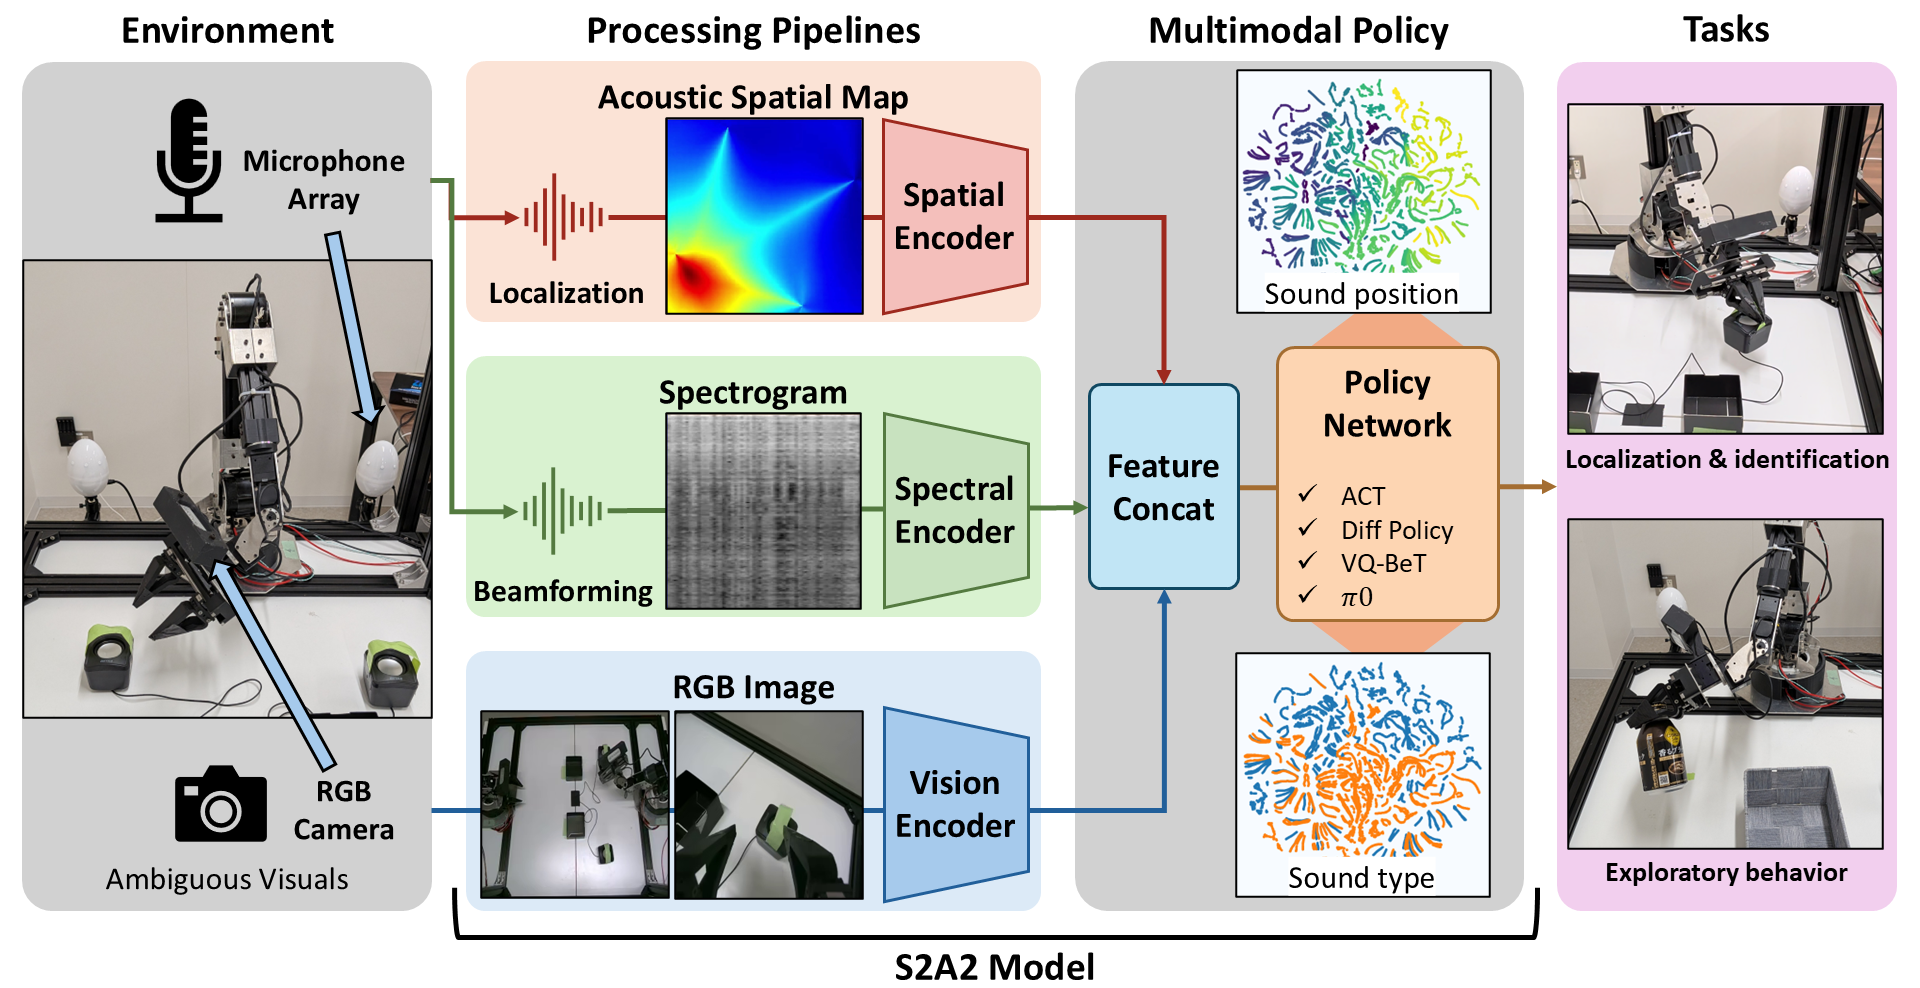
\includegraphics[keepaspectratio, width=14cm]{fig/fig1.png}
		\caption{The Overview of S2A2.
		RGBカメラから得られる画像はVision Encoderによって特徴量を抽出される．同様に，複数のマイクロフォンアレイから得られる多チャンネル音響信号からは，Acoustic Spatial MapとSpectrogramを生成し，それぞれ専用エンコーダで特徴量化する．これらの画像，音響特徴量を統合し，ACT，Diffusion Policy，VQ-BeT，$\pi_0$の4種の模倣学習Policyへ入力することで，音の識別であったり音の探索といった行動生成を可能にする．}
		\label{fig:fig1}
	\end{figure}

%===============================================================================
\section{Related Work}
	本研究は，模倣学習，manipulation with acoustic modality，robot audition with microphonearray processingの3領域にまたがるため，
	本節では，これらの各領域における関連研究について述べる．

\subsection{Imitation Learning and Multimodal Manipulation}
人間のデモンストレーションから直接Policyを学習する模倣学習は，ロボットが複雑な操作技能を獲得するための基本的な枠組みとして広く研究されてきた~\citep{pomerleau1988alvinn,argall2009survey,osa2018algorithmic}．
近年の深層模倣学習では，高次元な観測から連続的な行動系列を生成するために，方策の表現力を高める研究が進んでいる~\citep{rmp_survey2025}．
例えば，ACT~\citep{act}はTransformer~\citep{vaswani2017attention}と条件付きVAEを用いて行動系列をチャンクとして予測し，少数のデモンストレーションから接触に富む双腕操作を学習できることを示した．
Diffusion Policy~\citep{diffusionpolicy}は画像生成で発展した拡散モデル~\citep{ho2020ddpm}を行動生成に導入し，マルチモーダルな行動分布を逐次的なdenoising過程として表現する．
VQ-BeT~\citep{vqbet}は，連続行動を離散コードへ量子化し，Decoder-only Transformerによって自己回帰的に予測することで，長期的な行動構造を扱う．
また，$\pi_0$~\citep{pi0}はPaliGemma~\citep{beyer2024paligemma}を基盤とし，flow matching~\citep{lipman2023flow}によって行動系列を生成する．
これらの研究は，行動の時間構造や分布のマルチモダリティを扱う方策表現において多くの研究の基盤となる方策学習手法である．

一方で，方策が利用する入力モダリティという観点では，多くの手法は視覚情報を主入力としており，視覚に加えて言語を入力する大規模なVision-Language-Actionモデルもこの流れに位置づけられ，RT-2~\citep{brohan2023rt2}やOpenVLA~\citep{kim2024openvla}は，視覚と言語によるタスク指定を行動生成へ接続することで，汎用的な操作方策の学習を目指している~\citep{vla_survey2025}．
このような視覚・言語を用いた方策は，対象物やタスク目標が画像や言語指示として明示的に与えられる状況では強力である．
一方で，操作に必要な情報が外観に現れない場合や，外観上区別できない複数物体の中から対象を選択する場合には，視覚・言語だけでは環境中の物理的な曖昧性を十分に解消できない．

この制約を緩和するため，視覚以外のセンサモダリティを模倣学習へ統合する研究も進んでいる．
特に触覚は，接触後の力学的状態や局所的な物体情報を捉えるモダリティとして有効であり，視触覚を統合したpolicyは，密なパッキング~\citep{seehearfeel}，接触に富む操作~\citep{vtt2022,sts_il2024,vitamin2024,tacthru2025}，掌上での操作~\citep{neuralfeels2024}などにおいて，視覚のみのPolicyを上回ることが報告されている．
触覚や言語のモダリティと本研究で扱う音響表現は競合するものではないため，将来的にこれらの技術と組み合わせることでさらに多くのモダリティへと拡張できる可能性がある．

% 	人間のデモンストレーションから直接Policyを学習する模倣学習は，ALVINN~\citep{pomerleau1988alvinn}以来ロボット学習の枠組みとして用いられてきた~\citep{argall2009survey,osa2018algorithmic,rmp_survey2025}．
% 	近年では，行動分布のマルチモダリティをTransformer~\citep{vaswani2017attention}と条件付きVAEで扱うACT~\citep{act}が，低コストな双腕システム上で接触に富む操作を少数のデモンストレーションから学習できることを示した．
% 	Diffusion Policy~\citep{diffusionpolicy}は画像生成における拡散モデル~\citep{ho2020ddpm}を方策学習に転用し，VQ-BeT~\citep{vqbet}は行動を離散コードに量子化して自己回帰型のDecoder-only Transformerで予測する．
% 	より大規模なVision-Language-Action (VLA) モデルとしては，RT-2~\citep{brohan2023rt2}，OpenVLA~\citep{kim2024openvla}，	そしてPaliGemma~\citep{beyer2024paligemma}を基盤にflow matching~\citep{lipman2023flow}で行動列を生成する$\pi_0$~\citep{pi0}などがある．
% 	これらのPolicyはResNet~\citep{he2016resnet}系のバックボーンや事前学習済みのVLMを用い，主たる入力としてRGB画像に依存している．

% 	視覚以外のモダリティとしては触覚の利用が進んでおり，視触覚を統合したPolicyは密なパッキング~\citep{seehearfeel}，接触に富む操作~\citep{vtt2022,sts_il2024,vitamin2024,tacthru2025}，	掌上での操作~\citep{neuralfeels2024}において視覚のみのPolicyを上回ることが報告されている．
% 	% 本研究は，これら4種のポリシーを共通の比較対象としつつ，触覚ではなく音響モダリティ，とりわけ空間情報と周波数情報を	明示的に分離した音響表現を統合した際の挙動を体系的に検証する．

% %また，RT-2~\citep{brohan2023rt2}やOpenVLA~\citep{kim2024openvla}に代表される大規模Vision-Language-Action（VLA）モデル~\citep{vla_survey2025}は，視覚と言語を介して汎用的な操作能力を獲得する方向へ研究を拡張している．
\subsection{Manipulation with Acoustic Modality}
音響モダリティは，材料識別~\citep{eppe2018interactive,jin2019openenv}，
粒状物質の流量や量の推定~\citep{clarke2018learning,wilson2019pouring}，
液体の高さ推定~\citep{liang2020audiopouring,du2021robotpouring}など，
多くの認識タスクにおいて重要なモダリティとして用いられてきた．
音響モダリティのロボットへの直接的な応用としては，接触音を用いた方策学習\citep{seehearfeel,maniwav}や動作生成~\citep{thatsoundsright}が提案されており，接触音の有用性から大規模音響データセットによる事前学習\citep{hearingtouch2024}やVLAと組み合わせた先進的な手法\citep{audiovla}も研究されている．
%Hearing Touch~\citep{hearingtouch2024}は大規模音響データセットによる事前学習を接触音表現に転用し，	ManiWAV~\citep{maniwav}はear-in-hand型の音響・視覚デモを用いて実環境での接触操作を学習する．


%Hearing Touch~\citep{hearingtouch2024}は大規模音響データセットによる事前学習を接触音表現に転用し，	ManiWAV~\citep{maniwav}はear-in-hand型の音響・視覚デモを用いて実環境での接触操作を学習する．
接触音というよりも音響信号に着目した研究として，The Sound of Simulation~\citep{multigen2025}は生成モデルにより音響データを拡張したsim-to-realによる方策学習を，CAVER~\citep{caver2025}とMOSAIC~\citep{mosaic2024}は能動的探索と音響表現の組み合わせを扱う．
また，Play it by Ear~\citep{playitbyear}は遮蔽下の操作で視覚と音を併用している．

%VLAと組み合わせた先進的な研究としては，Audio-VLA~\citep{audiovla}はVLAモデルへ接触音を導入することで操作過程の動的フィードバックを扱う．VLAS~\citep{vlas2024}は音声指令をVLAへ取り込む方向性を提案している．
以上のような背景から，既存研究のほとんどは，グリッパ近傍や接触マイクから得られる単一チャンネルの音を用いており，マイクロフォンアレイを用いて音環境を空間的にとらえたモダリティに関しては限定的である．
% 音源の空間情報と周波数情報を明示的に分離してそれぞれの寄与を体系的に検証するものではない点で，本研究とは異なる．

\subsection{Robot Audition and Microphonearray Processing}
ロボット聴覚の分野では，ロボットが活動する環境ノイズ化においてマイクロフォンアレイを用いて音源定位・追跡・分離を実現する研究がされてきた~\citep{nakadai2020robotaudition,robotaudition_review2025}．
それに関連して，複数のマイクロフォンアレイを用いる研究も多くされており，非同期なマイクロフォンアレイを使用してのキャリブレーション~\citep{wang2024slamcalib}，仮想空間での音響シーンの再現\cite{gabriel20192d}，音源の追跡\citep{yamada2020sound}などが行われている．
特に，複数アレイとNMFを組み合わせたSpotforming~\citep{spotforming_nmf}は，対象領域に対応する音源を強調し，周囲雑音や同方向雑音を抑制する枠組みを提供する．
本研究は，これらのロボット聴覚技術をマニピュレーション模倣学習の文脈に接続した最初の研究であるとも位置付けることができる．
	%	音響SLAM~\citep{jin2024audioslam}
	%Bregmanの聴覚情景分析~\citep{bregman1990asa}に始まる流れの中で，
	%Schmidtによって提案されたMUSIC法~\citep{schmidt1986music}は高分解能なDOA推定の代表的手法であり~\citep{doa_survey2025}，の基盤としても用いられる．
	%統合的な聴覚処理基盤としてはHARK~\citep{nakadai2010hark}が広く知られ，
	%，	NMFに基づく多チャンネル音源分離~\citep{lee1999nmf,sekiguchi2019mnmf,shon2017nmf_doa}
	%マイクロフォンアレイ定位~\citep{valin2004ssl}や音源分離~\citep{valin2007postfilter}など，音響処理のための手段が蓄積されている．

	%これらの研究の主な評価対象は定位精度・分離性能・音声認識の前処理であり，得られた空間・周波数表現をPolicyの入力としてどのように使うかは十分には検討されてこなかった．
	% 本研究は，既存のロボット聴覚技術をマニピュレーション学習の文脈に接続し，Acoustic Spatial Mapを空間情報，Spotforming/NMF後のSpectrogramを周波数情報として用いることで，音が操作判断に与える役割を体系的に評価する．

% \subsection{本研究の位置づけ}
% 	以上の3領域を踏まえ，本研究と既存研究の違いを整理する．
% 	模倣学習の文脈では，視覚や触覚に加えて音響モダリティを扱う研究が増えつつあるが，音は主に接触マイクや単一マイクから得られるSpectrogramとして利用されており，	空間情報と周波数情報がPolicyの判断にそれぞれどう寄与するかは検討されていない．
% 	音響マニピュレーションの研究においても，音は接触イベントや状態変化の手がかりとして扱われることが多く，	外観が同一の複数物体を音源位置と音色の両方で識別するタスクは設定されていない．
% 	ロボット聴覚の分野では高精度な音源定位・分離技術が蓄積されているが，それらをPolicyの入力表現として活用する研究は限られている．
% 	本研究は，これら3領域の間隙を埋めるものである．
% 	具体的には，ロボット聴覚の空間音響処理（MUSIC法，Spotforming/NMF）を模倣学習の入力表現として再定式化し，空間情報と周波数情報を明示的に分離した上で，4タスク $\times$ 4 Policyの体系的評価により	各モダリティの寄与を定量的に検証する．

%===============================================================================






\section{Spatial-Spectral Audio Action (S2A2) Framework}
\label{sec:s2a2_framework}
	本章では，提案するSpatial-Spectral Audio Action (S2A2) Frameworkについて述べる．
	S2A2 Frameworkは，音響情報が操作判断に不可欠な環境において，ロボットが視覚，音響，および自己状態を統合し，適切な操作行動を生成するためのマルチモーダル模倣学習フレームワークである．

	Fig.~\ref{fig:fig1}に示すように，S2A2 Frameworkは，環境設定，S2A2 Model，およびAcoustic-Aware Manipulation Tasksから構成される．
	S2A2 Modelは，観測からモダリティ別特徴量を抽出するProcessing Pipelinesと，それらをProprioceptionと統合して行動を出力するMultimodal Policyからなる．
	
	本章の構成は以下の通りである．
	まず，Section~\ref{sec:problem}でS2A2 Frameworkの問題設定および模倣学習としての数理的定式化を定義する．
	次に，Section~\ref{sec:tasks}で本研究が対象とする具体的なタスクについて述べる．
	Section~\ref{sec:pipelines}では，S2A2 Modelを構成する3つのProcessing Pipelinesにおける前処理アルゴリズムとエンコーダの構造を説明する．
	最後に，Section~\ref{sec:policy}でMultimodal Policyによる特徴量統合と行動生成ついて述べる．




\subsection{Problem Formulation}
\label{sec:problem}
	S2A2 Frameworkは，Section~\ref{sec:tasks}でAcoustic-Aware Manipulation Tasksとして定義される，視覚のみでは正しい操作対象や搬送先を一意に決定できない環境におけるマニピュレーションタスクを対象とする．
	このような環境では，ロボットは物体の見た目だけでなく，音源の位置情報や音色を利用して行動を決定する必要がある．

	S2A2 Frameworkでは，この問題をマルチモーダル観測に条件づけられた模倣学習問題として定式化する．
	各時刻$t$における観測$o_t$は，RGB画像$I_t$，Acoustic Spatial Map$S_t$，Spectrogram$G_t$，およびProprioception$s_t$から構成される．

	\begin{equation}
	o_t = {I_t, S_t, G_t, s_t}
	\end{equation}

	S2A2 Modelは，これらの観測から行動$a_t$または将来の行動列$a_{t:t+H-1}$を予測するPolicy $\pi_\theta$を学習する．

	データセットをエキスパートによる観測・行動軌道 $\mathcal{D}=\{(o_t,a_t)\}$ とすると，学習の目的は次の模倣学習損失を最小化することである．

	\begin{equation}
	\min_{\theta}\ \mathbb{E}_{(o_t,a_t)\sim\mathcal{D}}
	\left[\mathcal{L}_{\mathrm{BC}}\left(\pi_\theta(o_t),a_t\right)\right],
	\end{equation}

	ここで $\theta$ はPolicyの学習パラメータ，$\mathbb{E}_{(o_t,a_t)\sim\mathcal{D}}[\cdot]$ はデータセット $\mathcal{D}$ からサンプルした観測・行動ペアに関する期待値，$\pi_\theta(o_t)$ はPolicyが観測 $o_t$ から予測する行動，$\mathcal{L}_{\mathrm{BC}}$ はエキスパート行動とのずれを測る模倣学習損失である．
	具体的な損失関数はPolicy Networkに依存し，その詳細はSection~\ref{sec:policy}およびAppendix~\ref{sec:appendix_architecture}で述べる．




\subsection{Acoustic-Aware Manipulation Tasks}
\label{sec:tasks}
	本研究では，音響情報が操作判断に果たす役割を体系的に評価するため，タスク達成に必要な音響情報が異なる4種類のマニピュレーションタスクを設計した．
	これらを総称してAcoustic-Aware Manipulation Tasksと呼ぶ．
	各タスクの概要をTable~\ref{tab:tasks}に示す．

	\textbf{Localization Task}では，環境に視覚的に同一の2つの物体と，1つの箱が配置される．
	このとき，2つの物体の初期位置はランダムであり，箱の初期位置は固定される．
	2つの物体のうち片方が常に音を発するので，その物体を把持して箱に入れるタスクである．
	発せられる音色は常に同一であり，把持対象の物体を選択するのに必要なのは，音源の空間情報である．
	このタスクは，Acoustic Spatial Mapが操作対象の定位に寄与するかを検証するために設計した．

	\textbf{Identification Task}では，環境に1つの物体と，2つの箱が配置される．
	このとき，物体の初期位置はランダムであり，箱の初期位置は固定される．
	物体は常に2種類の音のいずれかを発するので，その音色に応じて2種類の箱のうち対応する方へ搬送するタスクである．
	音を発する物体は1つであるため，視覚情報を用いれば把持対象の特定に音源の空間情報は不要である．
	一方で，正しく搬送先の箱を選択するためには音色識別が重要となる．
	このタスクは，Spectrogramが音源の音色識別に寄与するかを検証するために設計した．

	\textbf{Localization \& Identification Task}は，Localization TaskとIdentification Taskを複合した設計になっており，環境に視覚的に同一の2つの物体と，2つの箱が配置される．
	このとき，2つの物体の初期位置はランダムであり，箱の初期位置は固定される．
	2つの物体のうち，片方が常に音を発するので，その物体を把持する．
	この時，物体は2種類の音のいずれかを発しているので，その音色に応じて2種類の箱のうち対応する方へ搬送するタスクである．
	対象物体の選択には音源の空間情報が必要であり，搬送先の選択には音色識別が必要である．
	したがって，本タスクはAcoustic Spatial MapとSpectrogramの統合的利用を評価するために設計した．

	\textbf{Exploratory Task}では，環境に視覚的に同一の2つの物体と，1つの箱が配置される．
	このとき，2つの物体の初期位置はランダムであり，箱の初期位置は固定される．
	いずれの物体も静止時は音を発さず，片方だけが移動時に音を発するという設定で，音が鳴った方の物体を箱に入れるタスクである．
	そのため，マニピュレータは2つの物体を順に把持して振り，音が鳴るかどうかを確認するという探索行動を行う必要がある点，および把持後の音響フィードバックに応じて行動を分岐する必要がある点で，他の3タスクと異なる．

	\begin{table*}[t]
		\centering
		\scriptsize
		\setlength{\tabcolsep}{3pt}
		\caption{Acoustic-Aware Manipulation Task の概要と各タスクが要求する音響的能力．L \& I TaskはLocalization \& Identification Taskの略称である．}
		\label{tab:tasks}
		\begin{tabular}{p{0.10\textwidth} p{0.54\textwidth} >{\centering\arraybackslash}p{0.09\textwidth} >{\centering\arraybackslash}p{0.09\textwidth} >{\centering\arraybackslash}p{0.09\textwidth}}
			\hline
			Task & 説明 & 音の位置情報 & 音の種類識別 & 探索的行動 \\
			\hline
			Localization Task & 音を発している物体を定位し，把持して箱へ搬送する． & $\checkmark$ & -- & -- \\
			Identification Task & 音色を識別し，対応する箱へ物体を分類する． & -- & $\checkmark$ & -- \\
			L \& I Task & 音源位置に基づき対象物体を選び，音色に基づき搬送先を決定する． & $\checkmark$ & $\checkmark$ & -- \\
			Exploratory Task & 物体を振って音響フィードバックを取得し，音が鳴る物体を搬送する． & $\checkmark$ & $\checkmark$ & $\checkmark$ \\
			\hline
		\end{tabular}
	\end{table*}




\subsection{Processing Pipeline}
\label{sec:pipelines}
S2A2 Modelの3つのProcessing Pipelinesは，入力モダリティごとに異なる前処理アルゴリズムとエンコーダを持つ．
Acoustic Spatial Map Pipelineは多チャンネル音響信号から空間音響表現を生成し，Spatial Encoderで特徴量化する．
Spectrogram Pipelineは目的音源を強調したSpectrogramを生成し，Spectral Encoderで特徴量化する．
RGB Image Pipelineは2台のカメラから取得したRGB画像をVision Encoderで特徴量化する．
以下では，各PolicyのVision Encoderを直接利用するRGB Image Pipelineを除いた，Acoustic Spatial Map PipelineとSpectrogram Pipelineについて述べる．




\subsubsection{Acoustic Spatial Map Pipeline}
\label{sec:doa}
	Acoustic Spatial Map Pipelineでは，まず多チャンネル音響信号から音源方向の尤度を推定し，それを作業空間に対応する二次元マップへ投影する．
	具体的には各マイクロフォンアレイの多チャンネル信号に対し，MUSIC（MUltiple SIgnal Classification）法~\citep{schmidt1986music}を適用する．
	入力音声信号はサンプリング周波数16kHzで取得し，FFT長512，50\%オーバーラップの短時間フーリエ変換 (STFT) で周波数領域へ変換する．
	$c\in\{1,\ldots,n\}$ をアレイのインデックス，$M$ を各アレイのマイクロフォン数とする．
	$c$ 番目のアレイで観測された $M$ チャンネル信号のSTFTを $\mathbf{x}_{c,f,\tau}\in\mathbb{C}^{M}$ とすると，周波数ビン $f$ における空間共分散行列は式 \ref{eq:eq_a} で与えられる．

	\begin{equation}
	\label{eq:eq_a}
	\mathbf{R}_{c,f}=\frac{1}{T}\sum_{\tau=1}^{T}
	\mathbf{x}_{c,f,\tau}\mathbf{x}_{c,f,\tau}^{\mathrm{H}}
	\end{equation}
	
	ここで $\mathbb{C}^{M}$ は $M$ 次元複素ベクトル空間，$\mathbf{R}_{c,f}$ は $c$ 番目のアレイにおける周波数ビン $f$ の空間共分散行列，$T$ はSTFTの時間フレーム数，$\tau$ は時間フレームのインデックス，$\mathrm{H}$ は複素共役転置を表す．

	MUSIC法は，$\mathbf{R}_{c,f}$ の固有値分解から雑音部分空間 $\mathbf{E}_{n,c,f}$ を求め，方向 $\theta$ のステアリングベクトル $\mathbf{a}_{c,f}(\theta)$ との直交性に基づいて，式 \ref{eq:eq_b} で空間スペクトルを計算する．

	\begin{equation}
	\label{eq:eq_b}
	P_c(\theta)=\frac{1}{|\mathcal{F}|}\sum_{f\in\mathcal{F}}
	\frac{1}{\mathbf{a}_{c,f}(\theta)^{\mathrm{H}}
	\mathbf{E}_{n,c,f}\mathbf{E}_{n,c,f}^{\mathrm{H}}
	\mathbf{a}_{c,f}(\theta)}
	\end{equation}
	
	ここで $\mathbf{E}_{n,c,f}$ は雑音部分空間を張る固有ベクトルを列に持つ行列，添字 $n$ はnoise subspaceを表す．$\mathcal{F}$ は平均化に用いる周波数ビン集合，$|\mathcal{F}|$ はその要素数である．

	方位ごとの空間スペクトルを対数化および正規化した値をDOAスコアとし，これを作業空間のマイクロフォンアレイが存在する平面に対応した $224\times224$ の二次元平面へ投影し，$n$ チャンネルのAcoustic Spatial Mapを生成する．
	画像の行インデックスを $i$，列インデックスを $j$ とし，画像座標 $u=(i,j)$ に対応する作業空間上の点を $p(u)$，アレイ中心を $m_c$ とすると，各チャンネルの値は式 \ref{eq:eq_c} で計算される．

	\begin{equation}
	\label{eq:eq_c}
	S_c(u)=\frac{\bar{P}_c(\theta(p(u),m_c))}
	{\left(\|p(u)-m_c\|_2+d_{\mathrm{floor}}\right)^\gamma}
	\end{equation}
	
	ここで $\bar{P}_c$ は正規化後のDOAスコア，$\theta(p(u),m_c)$ は $m_c$ から $p(u)$ へ向かう方位角，$\|\cdot\|_2$ はユークリッド距離，$d_{\mathrm{floor}}$ と $\gamma$ は距離減衰を安定化するパラメータである．

	全アレイの $S_c$ を重ねた多チャンネルマップ $S\in\mathbb{R}^{224\times224\times n}$ を最終的なAcoustic Spatial Mapとして用いる．
	ここで $\mathbb{R}$ は実数の集合である．
	% Policyへ入力するAcoustic Spatial Mapは $S$ の $n$ チャンネルであり，本研究の標準設定では $n=4$ とする．
	% この表現は，単一の推定座標に情報を圧縮せず，各アレイから見た方向尤度を保持するため，視覚特徴との空間的な対応づけを学習しやすい．
	このAcoustic Spatial Map $S$ を，Spatial Encoder に入力し，Policy Network が利用できる特徴量に変換する．
	Acoustic Spatial Map は，通常の RGB 画像とは異なり，入力チャンネル数や値の統計分布が異なる．
	そのため，各Policy NetworkのVision Encoderとは重みを共有せず，Acoustic Spatial Map専用のEncoderを用いる．

	Spatial Encoder の backbone には，入力チャンネル数を $n$ に拡張した ResNet 型 CNN を用いて，出力としてfeature mapを得る．




\subsubsection{Spectrogram Pipeline}
\label{sec:spec}
	Spectrogram Pipelineは，Acoustic Spatial Mapでは捉えにくい音色などの周波数情報を抽出するためのpipelineである．
	本研究ではSpotforming~\citep{spotforming_nmf}に基づき，目的音源方向の強調とNMF~\citep{lee1999nmf}による共通成分抽出を組み合わせ，雑音やサイドローブを抑制したSpectrogramを生成する．

	% まず全アレイのマップを式 \ref{eq:eq_d} として統合し，ガウシアンフィルタ（$\sigma=1.0$）を適用した後，局所最大点を音源候補として選択する．
	まず全アレイのマップを式 \ref{eq:eq_d} として統合し，ガウシアンフィルタを適用した後，局所最大点を音源候補として選択する．
	
	\begin{equation}
	\label{eq:eq_d}
	S_{\mathrm{sum}}(u)=\sum_{c=1}^{n} S_c(u)
	\end{equation}

	本研究で扱うタスクは，同時に存在する音源の数が1つであるため，音源候補は最大で1とした．
	また$S_{\mathrm{sum}}$ は全アレイを統合した音源候補マップである．

	選択された音源候補を各アレイから見た方位を $\hat{\theta}_c$ とし，各アレイでは $\hat{\theta}_c$ に合わせて，音の時刻のずれを補正するDelay-and-Sumビームフォーミングを行う．
	
	\begin{equation}
	\label{eq:eq_e}
	y_c(t)=\frac{1}{M}\sum_{m=1}^{M}
	x_{c,m}(t-\tau_{c,m}(\hat{\theta}_c)).
	\end{equation}

	ここで $t$ は時刻，$x_{c,m}(t)$ は $c$ 番目のアレイの $m$ 番目のマイクロフォン信号，$\tau_{c,m}(\hat{\theta}_c)$ は方位 $\hat{\theta}_c$ から到来する音が各マイクに届くまでの相対遅延である．

	次に各アレイのビームフォーミング出力 $y_c$ の振幅Spectrogramを時間方向に結合した非負値行列 $\mathbf{V}\in\mathbb{R}_{\ge0}^{F_b\times nT_b}$ を作る．
	ここで $F_b$ は周波数ビン数，$T_b$ は各アレイの時間フレーム数である．$\mathbf{V}$ を50成分のNMFにより式 \ref{eq:eq_f} のように分解する．
	
	\begin{equation}
	\label{eq:eq_f}
	\mathbf{V}\approx \mathbf{W}\mathbf{H},\quad
	\mathbf{W}\ge0,\ \mathbf{H}\ge0
	\end{equation}
	
	ここで $\mathbb{R}_{\ge0}$ は非負実数の集合，$\mathbf{W}\in\mathbb{R}_{\ge0}^{F_b\times R}$ は基底行列，$\mathbf{H}\in\mathbb{R}_{\ge0}^{R\times nT_b}$ は活性行列，$R=50$ はNMF成分数である．

	活性行列をアレイごとの時間区間に分割したものを $\mathbf{H}^{(c)}\in\mathbb{R}_{\ge0}^{R\times T_b}$ とし，各アレイで共通して強い成分を式 \ref{eq:eq_g} として推定する．

	\begin{equation}
	\label{eq:eq_g}
	\mathbf{Z}=\min_{c}\mathbf{H}^{(c)}
	\end{equation}
	
	ここで $\min_c$ は各NMF成分・各時刻についてアレイ方向の最小値を取る演算である．

	$\mathbf{Z}$ を最大値で正規化した行列を $\tilde{\mathbf{Z}}$ とし，閾値 $\delta=1.6\times10^{-3}$ によるバイナリマスク $\mathbf{B}$ を式 \ref{eq:eq_h} として作成する．

	\begin{equation}
	\label{eq:eq_h}
	\mathbf{B}_{r,\tau}=
	\begin{cases}
	1 & \tilde{\mathbf{Z}}_{r,\tau}>\delta,\\
	0 & \mathrm{otherwise}
	\end{cases}
	\end{equation}
	
	ここで $r$ はNMF成分のインデックス，$\tau$ はNMF活性行列における時間フレームのインデックス，$\mathbf{B}_{r,\tau}=1$ はその成分を再構成に残すことを表す．
	本研究ではマスクが広がりすぎることを避けるため，$\mathbf{B}$ の非ゼロ比率が0.2を超える場合は上位20\%の活性のみを残すように閾値を適応的に引き上げる．

	最後に $\mathbf{W}(\mathbf{H}^{(c)}\odot\mathbf{B})$ により各アレイの振幅Spectrogramを再構成する．
	ここで $\odot$ は要素ごとの積である．

	位相には同じアレイのビームフォーミング出力 $y_c$ のSTFT位相を用い，逆STFTで得た波形をアレイ間で平均する．この処理は，目的音源が全アレイで観測される一方，サイドローブや局所雑音は一部のアレイでのみ強く現れるという仮定に基づく．

	NMFで抽出した共通成分を再構成・統合し，雑音を抑制した単一チャンネルの対数パワーSpectrogramを生成する．
	再構成波形 $\hat{y}(t)$ のSTFTを $\hat{Y}_{f,\tau}$ とすると，Spectrogram画像は式 \ref{eq:eq_i} として計算する．

	\begin{equation}
	\label{eq:eq_i}
	G(f,\tau)=10\log_{10}\left(|\hat{Y}_{f,\tau}|^2+\epsilon\right)
	\end{equation}
	
	ここで $f$ は周波数ビン，$\tau$ は時間フレーム，$\epsilon=10^{-10}$ は対数計算を安定化する微小正数である．
	表示周波数帯域と画像化時の正規化はシミュレーション評価と実機評価で異なり，具体的な値はAppendix~\ref{sec:appendix_sim_real}に示す．

	このSpectrogram $G$ を，Spectral Encoder に入力し，Policy Network が利用できる特徴量に変換する．
	Spatial Encoderと同様に，Spectral EncoderもPolicy Network の Vision Encoder とは重みを共有せず，Spectrogram専用のEncoderを用いる．
	Spectral Encoderのbackboneには，入力チャンネル数を1に変更したResNet型CNNを用いて，出力としてfeature mapを得る．





\subsection{Multimodal Policy}
\label{sec:policy}
論文のMethodセクションの下書きですね。コメントアウトされていた詳細で正確な記述（数式、各変数の定義、具体的なパラメータや学習手順など）を全面的に採用し、学術論文としてより洗練された自然な日本語になるように全体を修正・統合しました。

以下が修正後の文章です。そのままコピーしてご活用いただけます。

---

\subsection{Multimodal Policy}
\label{sec:policy}
	Multimodal Policyは，Processing Pipelinesから抽出された各モダリティの特徴量とProprioceptionを統合し，ロボットの行動を生成するモジュールである．

	本研究では，行動生成を行うPolicy NetworkとしてACT~\citep{act}，Diffusion Policy~\citep{diffusionpolicy}，VQ-BeT~\citep{vqbet}，および$\pi_0$~\citep{pi0}の4種類を採用した．
	主要な設計方針として，これらの既存Policy Networkの基本アーキテクチャを大きく変更することなく，音響表現を各Policyが扱えるトークンまたは条件ベクトルへ変換し，RGB画像やProprioceptionとシームレスに統合できるように拡張を施している．

	Section~\ref{sec:pipelines}で述べたように，各Pipelineは共通の形式としてFeature Mapを出力する．
	一方で，得られたFeature MapをPolicy Networkへ入力する形式は，各Policyの構造に応じて以下のように異なる．
	ACTおよび$\pi_0$では，Feature Mapを$1\times1$ convolutionによってPolicyの隠れ次元へ射影する．
	その後，Feature Map上の各空間位置を1つの独立したトークンとして扱い，Positional Embeddingを加算したトークン列としてPolicy Networkに入力する．
	Diffusion PolicyおよびVQ-BeTでは，Feature Mapを$n_{key}$チャンネルを持つ2次元マップへ射影する．
	次に，各チャンネルに対して空間方向にSoftmaxを適用し，各空間位置の重みを算出する．
	この重みに基づいて，正規化されたFeature Map座標の重み付き平均を計算することで各チャンネルのKeypoint特徴を抽出し，最後にこれらをFlattenして1次元のベクトルへと変換してからPolicy Networkに入力する．

	各Policy Networkは，上記の手順で統合された特徴量を用いて，以下の通り，学習および推論を行う．

	ACTでは，RGB画像，Acoustic Spatial Map，およびSpectrogramから抽出したトークン列に，Proprioceptionを状態トークンとして加え，Transformer encoderへ入力する．
	Decoderは長さ$H_{\mathrm{act}}$のaction chunkを出力する．
	訓練時にはVAEを併用し，式 \ref{eq:eq_j} の損失関数を最小化する．

	\begin{equation}
	\label{eq:eq_j}
	\mathcal{L}_{\mathrm{ACT}} = \frac{1}{H_{\mathrm{act}} d_a}\sum_{h=0}^{H_{\mathrm{act}}-1} m_h\left\|\hat{a}_{t+h}-a_{t+h}\right\|_1 + \beta_{\mathrm{KL}}\, D_{\mathrm{KL}}\left(q_\phi(z\mid a_{t:t+H_{\mathrm{act}}-1},s_t)\,\|\,\mathcal{N}(0,\mathbf{I})\right)
	\end{equation}

	ここで，$d_a$は行動の次元数，$h$はaction chunk内の時刻インデックス，$\hat{a}_{t+h}$および$a_{t+h}$はそれぞれ予測行動とエキスパート行動である．
	$m_h\in\{0,1\}$はデータ列端のパディングを損失計算から除外するためのマスク，$s_t$はProprioception，$z$はVAEの潜在変数，$\phi$はVAE encoderのパラメータ，$q_\phi$は出力される潜在分布を示す．
	また，$\mathcal{N}(0,\mathbf{I})$は平均$0$・共分散が単位行列の標準正規分布，$D_{\mathrm{KL}}$はKLダイバージェンスであり，KL項の重みは$\beta_{\mathrm{KL}}=10$とした．

	Diffusion Policyでは，各Pipelineから得た特徴量とProprioceptionを結合し，U-Netのグローバル条件ベクトルとして用いる．
	訓練では，長さ$H_d=16$の行動列$x_0=a_{t-1:t+14}$に対し，100段階の拡散ステップから一様にサンプルしたステップ$k$において，ノイズ$\epsilon\sim\mathcal{N}(0,\mathbf{I})$を付加した$x_k$を式 \ref{eq:eq_k} で生成する．

	\begin{equation}
	\label{eq:eq_k}
	x_k=\sqrt{\bar{\alpha}_k}x_0+\sqrt{1-\bar{\alpha}_k}\epsilon
	\end{equation}

	ここで，$\bar{\alpha}*k$はDDPMのノイズスケジュールから定まる係数である．
	モデルであるU-Netを$\epsilon*\theta$，観測条件をエンコードしたベクトルを$g(o)$とすると，U-Netが付加ノイズを予測するように式 \ref{eq:eq_l} の損失関数を最小化する．

	\begin{equation}
	\label{eq:eq_l}
	\mathcal{L}_{\mathrm{Diff}} =\mathbb{E}_{x_0,\epsilon,k} \left[\frac{1}{H_d d_a}\left\|\epsilon_\theta(x_k,k,g(o))-\epsilon\right\|_2^2\right]
	\end{equation}

	ここで，$\theta$はU-Netの学習パラメータ，$o$は観測変数である．
	推論時には100ステップの逆拡散処理を行い，観測履歴の最終時刻から8ステップ分の行動を実行候補として出力する．

	VQ-BeTでは，各Pipelineの特徴量，Proprioception，およびAction Query TokenをDecoder-onlyのTransformerによるPolicy Networkへ入力する．
	行動出力の表現にはRQ-VAE~\citep{rqvae}を用い，長さ$5$のaction chunkを，あらかじめ各層のコードブックサイズが$16$である，2層の離散コードへと変換しておく．
	訓練時，Policy Networkは固定されたRQ-VAEに対し，各Action Query Tokenから離散コードの確率分布と連続的なオフセットを予測するように学習される．
	予測action chunkを$\hat{A}*j$，正解action chunkを$A_j$，1層目および2層目の正解コードをそれぞれ$c_j^{(1)}, c_j^{(2)}$，予測コード分布を$p*{\theta,j}^{(1)}, p_{\theta,j}^{(2)}$とすると，損失関数は式 \ref{eq:eq_m} として定義される．

	\begin{equation}
	\label{eq:eq_m}
	\mathcal{L}_{\mathrm{VQ}} =\frac{1}{J}\sum_{j=1}^{J}\left[ \lambda_{\mathrm{off}}\frac{1}{H_q d_a}\|\hat{A}_j-A_j\|_1 +\lambda_1\,\mathrm{FL}(p_{\theta,j}^{(1)},c_j^{(1)}) +\lambda_2\,\mathrm{FL}(p_{\theta,j}^{(2)},c_j^{(2)}) \right]
	\end{equation}

	ここで，$\theta$はPolicy Networkの学習パラメータ，$j$はAction Query Tokenのインデックス，$J=3$はTokenの総数，$H_q=5$は1つのTokenが担当するaction chunk長である．$\mathrm{FL}$はFocal Lossを表し，正解コード$c$に割り当てられた予測確率を$p_c$として式 \ref{eq:eq_n} で定義される．

	\begin{equation}
	\label{eq:eq_n}
	\mathrm{FL}(p,c)=-(1-p_c)^2\log p_c
	\end{equation}

	$\pi_0$では，RGB画像をSigLIPベースのEncoderでトークン化したものと，Acoustic Spatial MapとSpectrogramをトークン化したものをconcatenateし，Prefixに追加する．
	一方，Proprioception，ノイズ付き行動，および時刻埋め込みはSuffix側に入力される．
	なお，ここでPrefixとはVLM側のFFNにルーティングされるトークンのことを指し，SuffixとはAction Expert側のFFNにルーティングされるトークンのことを指す．
	本手法では，ノイズ分布からデータ分布へ移動する連続的な速度場を学習する生成手法であるFlow Matchingに基づきモデルを訓練する．
	正解行動列を$a$，同形状の標準正規ノイズを$\epsilon$，時刻を$r=0.999b+0.001$，$b\sim\mathrm{Beta}(1.5,1.0)$とし，式 \ref{eq:eq_o} で学習目標となる教師速度$u_r$を作成する．

	\begin{equation}
	\label{eq:eq_o}
	x_r=r\epsilon+(1-r)a,\qquad u_r=\epsilon-a
	\end{equation}

	そして，モデル$v_\theta$が教師速度$u_r$を予測するように，式 \ref{eq:eq_p} の損失関数を最小化する．

	\begin{equation}
	\label{eq:eq_p}
	\mathcal{L}_{\pi_0} =\mathbb{E}_{a,\epsilon,r} \left[\frac{1}{H_\pi d_a}\left\|v_\theta(x_r,r,o)-u_r\right\|_2^2\right]
	\end{equation}

	ここで，$\theta$は速度場モデルの学習パラメータ，$H_\pi=50$はaction chunk長，$x_r$はノイズ付き行動，$u_r$はノイズから正解行動へ向かう速度，そして$o$はPrefixとProprioceptionを含む観測条件である．なお，本実験ではPaliGemma側に事前学習済みの重みを使用し，音響エンコーダは追加モジュールとしてスクラッチから学習した．

	各Policy Networkの詳細なハイパーパラメータ，観測履歴長，action chunk長，正規化方法，および推論設定については，Appendix~\ref{sec:appendix_architecture}にまとめる．





	% Multimodal Policyは，Processing Pipelinesで得られた特徴量とProprioceptionを統合し，行動を出力する部分である．

	% 本研究では，行動生成Policy NetworkとしてACT~\citep{act}，Diffusion Policy~\citep{diffusionpolicy}，VQ-BeT~\citep{vqbet}，および$\pi_0$~\citep{pi0}の4種類を用いる．
	% 本研究では，これらのPolicy Networkのアーキテクチャを大きく変更することなく，音響表現を既存Policyが扱えるトークンまたは条件ベクトルへ変換し，RGB画像やProprioceptionと統合できるようにすることを主要な設計方針とした．

	% Section~\ref{sec:pipelines}で述べたように，各Pipelineは共通した形式としてfeature mapを出力する．
	% 一方で，各feature mapをPolicy Networkに渡す形式は，Policyによって異なる．

	% ACT および $\pi_0$ では，feature map を $1\times1$ convolution により Policy の隠れ次元へ射影する．
	% その後、feature map 上の各空間位置を1つのトークンとして扱い，位置埋め込みを加えたトークン列として Policy Network に入力する．

	% Diffusion Policy および VQ-BeT では，feature mapを$n_{key}$チャンネルを持つ2次元マップへ射影する．
	% 次に，各チャンネルについて空間方向にSoftmaxを適用し，各位置の重みを得る．
	% その重みに基づいて，正規化されたfeature map座標の重み付き平均を計算することで，各チャンネルのkeypoint特徴を得る．
	% 最後に，得られたkeypoint特徴をflattenしてベクトル化し，Policy Networkに入力する．

% この部分に何か文章を入れる．
% 上記の操作によって得られた特徴量を用いて各Policy Networkは学習および推論を行う．みたいな感じ．

	% ACTでは，RGB画像，Acoustic Spatial Map，Spectrogramから得たトークン列に加え，Proprioceptionを状態トークンとして追加し，Transformer encoderへ入力する．
	% decoderは長さ$H_{\mathrm{act}}$のaction chunkを出力する．
	% 訓練時にはVAEを併用し，action chunkのL1誤差と潜在変数のKLダイバージェンスを最小化する．

	% \begin{equation}
	% \mathcal{L}{\mathrm{ACT}}
	% =\frac{1}{H{\mathrm{act}}d_a}\sum_{h=0}^{H_{\mathrm{act}}-1}
	% m_h\left|\hat{a}{t+h}-a{t+h}\right|1
	% +\beta{\mathrm{KL}}D_{\mathrm{KL}}\left(q_\phi(z\mid a_{t:t+H_{\mathrm{act}}-1},s_t),|,\mathcal{N}(0,\mathbf{I})\right).
	% \end{equation}
	
	% ここで，$d_a$は行動次元，$m_h$はパディングを除外するマスク，$z$はVAEの潜在変数である．

% 	訓練損失は
% 	\begin{equation}
% 	\mathcal{L}_{\mathrm{ACT}}
% 	=\frac{1}{H_{act} d_a}\sum_{h=0}^{H_{act}-1}
% 	m_h\left\|\hat{a}_{t+h}-a_{t+h}\right\|_1
% 	+\beta_{\mathrm{KL}}\,
% 	D_{\mathrm{KL}}\left(q_\phi(z\mid a_{t:t+H_{act}-1},s_t)\,\|\,\mathcal{N}(0,\mathbf{I})\right)
% 	\end{equation}
% 	である．ここで $d_a$ は行動次元，$h$ は行動チャンク内の時刻インデックス，$\hat{a}_{t+h}$ は予測行動，$a_{t+h}$ はエキスパート行動，$m_h\in\{0,1\}$ はデータ列端のパディングを損失から除外するためのマスク，$s_t$ はProprioception，$z$ はVAEの潜在変数，$\phi$ はVAE encoderのパラメータ，$q_\phi$ はVAE encoderが出力する潜在分布，$\mathcal{N}(0,\mathbf{I})$ は平均0・共分散単位行列の標準正規分布，$D_{\mathrm{KL}}$ はKLダイバージェンス，$\beta_{\mathrm{KL}}=10$ はKL項の重みである．


	% Diffusion Policyでは，各pipelineから得た特徴量とProprioceptionをconcatし，U-Netのグローバル条件ベクトルとして用いる．訓練では，正解行動列$x_0$へ拡散ステップ$k$に応じたノイズ$\epsilon$を加えた$x_k$を入力し，U-Net $\epsilon_\theta$が付加ノイズを予測するように学習する：
	% \begin{equation}
	% \mathcal{L}{\mathrm{Diff}}
	% =\mathbb{E}{x_0,\epsilon,k}
	% \left[\frac{1}{H_d d_a}\left|\epsilon_\theta(x_k,k,g(o))-\epsilon\right|_2^2\right].
	% \end{equation}
	% ここで，$g(o)$は観測$o$をエンコードしてconcatした条件ベクトルである．
% 	訓練では，長さ $H_d=16$ の行動列 $x_0=a_{t-1:t+14}$ に対し，100段階の拡散ステップから一様にサンプルした $k$ でノイズ $\epsilon\sim\mathcal{N}(0,\mathbf{I})$ を加えた
% 	\begin{equation}
% 	x_k=\sqrt{\bar{\alpha}_k}x_0+\sqrt{1-\bar{\alpha}_k}\epsilon
% 	\end{equation}
% 	を作る．ここで $\bar{\alpha}_k$ はDDPMのノイズスケジュールから定まる係数である．U-Netを $\epsilon_\theta$，観測条件を $g(o)$ とすると，損失は
% 	\begin{equation}
% 	\mathcal{L}_{\mathrm{Diff}}
% 	=\mathbb{E}_{x_0,\epsilon,k}
% 	\left[\frac{1}{H_d d_a}\left\|\epsilon_\theta(x_k,k,g(o))-\epsilon\right\|_2^2\right]
% 	\end{equation}
% 	である．ここで $\theta$ はU-Netの学習パラメータ，$o$ は観測，$g(o)$ は観測をエンコードした条件ベクトル，$d_a$ は行動次元である．推論時は100ステップの逆拡散を行い，観測履歴の最後の時刻から8ステップ分の行動を実行候補として取り出す．

	% VQ-BeTでは，各pipeline特徴，Proprioception，およびaction query tokenをGPTスタイルのPolicy Networkへ入力する．VQ-VAEで行動チャンクを離散コードへ変換した後，Policy Networkは各action query tokenに対して離散コード確率と連続オフセットを予測する．損失は，オフセットのL1損失とコード分類のFocal Lossからなる：
	% \begin{equation}
	% \mathcal{L}{\mathrm{VQ}}
	% =\frac{1}{J}\sum{j=1}^{J}\left[
	% \lambda_{\mathrm{off}}\frac{1}{H_q d_a}|\hat{A}j-A_j|1
	% +\lambda_1\mathrm{FL}(p{\theta,j}^{(1)},c_j^{(1)})
	% +\lambda_2\mathrm{FL}(p{\theta,j}^{(2)},c_j^{(2)})
	% \right].
	% \end{equation}
% 	訓練は2段階で行う．第1段階ではResidual VQ-VAEを20,000ステップ学習し，長さ5の行動チャンクを2層のResidual Vector Quantization（RVQ）コードへ離散化する．
% 	RVQとは，1つ目のコードで粗い代表ベクトルを選び，2つ目以降のコードで残差を順に量子化する方法である．
% 	codebookとは離散コードが参照する代表ベクトルの集合であり，本研究では各RVQ層のcodebook sizeを16とした．
% 	第2段階では，固定したVQ-VAEに対して，policy networkがコード確率とオフセットを予測する．
% 	予測行動チャンクを $\hat{A}_j$，正解行動チャンクを $A_j$，1層目と2層目の正解コードをそれぞれ $c_j^{(1)},c_j^{(2)}$，予測コード分布を $p_{\theta,j}^{(1)},p_{\theta,j}^{(2)}$ とすると，損失は
% 	\begin{equation}
% 	\mathcal{L}_{\mathrm{VQ}}
% 	=\frac{1}{J}\sum_{j=1}^{J}\left[
% 	\lambda_{\mathrm{off}}\frac{1}{H_q d_a}\|\hat{A}_j-A_j\|_1
% 	+\lambda_1\,\mathrm{FL}(p_{\theta,j}^{(1)},c_j^{(1)})
% 	+\lambda_2\,\mathrm{FL}(p_{\theta,j}^{(2)},c_j^{(2)})
% 	\right]
% 	\end{equation}
% 	である．ここで $\theta$ はpolicy networkの学習パラメータ，$j$ はaction query tokenのインデックス，$J=3$ はaction query token数，$H_q=5$ は1つのaction query tokenが担当する行動チャンク長，$d_a$ は行動次元である．
% 	$\mathrm{FL}$ はFocal Lossであり，正解コード $c$ に割り当てられた確率を $p_c$ とすると
% 	\begin{equation}
% 	\mathrm{FL}(p,c)=-(1-p_c)^2\log p_c
% 	\end{equation}
% 	で定義される．

	% $\pi_0$では，RGB画像をPaliGemmaの画像エンコーダでトークン化し，Acoustic Spatial MapとSpectrogramは専用エンコーダで特徴マップ化した後，$1\times1$畳み込みでPaliGemmaの隠れ次元へ射影してprefixへ追加する．Proprioception，ノイズ付き行動，時刻埋め込みはsuffix側に入力される．flow matchingに基づき，正解行動列$a$，標準正規ノイズ$\epsilon$，時刻$r$に対して
	% \begin{equation}
	% x_r=r\epsilon+(1-r)a,\qquad u_r=\epsilon-a
	% \end{equation}
	% を作り，モデル$v_\theta$が速度$u_r$を予測するように
	% \begin{equation}
	% \mathcal{L}{\pi_0}
	% =\mathbb{E}{a,\epsilon,r}
	% \left[\frac{1}{H_\pi d_a}\left|v_\theta(x_r,r,o)-u_r\right|_2^2\right]
	% \end{equation}
	% を最小化する．
% 	flow matchingとは，ノイズ分布からデータ分布へ移動する連続的な速度場を学習する生成手法である．正解行動列を $a$，同じ形状の標準正規ノイズを $\epsilon$，時刻を $r=0.999b+0.001$，$b\sim\mathrm{Beta}(1.5,1.0)$ とすると，訓練時には
% 	\begin{equation}
% 	x_r=r\epsilon+(1-r)a,\qquad u_r=\epsilon-a
% 	\end{equation}
% 	を作り，モデル $v_\theta$ が速度 $u_r$ を予測するように
% 	\begin{equation}
% 	\mathcal{L}_{\pi_0}
% 	=\mathbb{E}_{a,\epsilon,r}
% 	\left[\frac{1}{H_\pi d_a}\left\|v_\theta(x_r,r,o)-u_r\right\|_2^2\right]
% 	\end{equation}
% 	を最小化する．ここで $\theta$ は速度場モデルの学習パラメータ，$H_\pi=50$ は行動チャンク長，$d_a$ は行動次元，$x_r$ はノイズ付き行動，$u_r$ はノイズから正解行動へ向かう教師速度，$o$ はprefixとProprioceptionを含む観測条件である．
% 	本実験ではPaliGemma側に事前学習済み重みを用い，音響エンコーダは追加モジュールとして学習した．

	% 各Policy Networkの詳細なハイパーパラメータ，観測履歴長，行動チャンク長，正規化方法，および推論設定はAppendix~\ref{sec:appendix_architecture}にまとめる．




% この文章は使えそうなら使う．要らなければ消す．
	% 本研究では行動生成Policyとして\textbf{ACT}~\citep{act}，\textbf{Diffusion Policy}~\citep{diffusionpolicy}，\textbf{VQ-BeT}~\citep{vqbet}，\textbf{$\pi_0$}~\citep{pi0} の4種を評価する．
	% 本研究のアーキテクチャ上の変更点は，各Policyの行動生成部を大きく変更するのではなく，Acoustic Spatial MapとSpectrogramを既存Policyが扱えるトークンまたは条件ベクトルへ変換する入力エンコーダを追加した点である．
	% 標準設定では，正面RGB画像，側面RGB画像，$n$ チャンネルAcoustic Spatial Map，1チャンネルSpectrogram，Proprioceptionを入力する．
	% Acoustic Spatial Mapは $n$ 個のマイクロフォンアレイに対応するチャンネルを持ち，本実験の標準設定では $n=4$ である．
	% SpectrogramはすべてのPolicyで1チャンネル入力として扱う．
	% 主要な学習パラメータを本文中の~\ref{sec:sim_setup}とAppendix~\ref{sec:appendixA}に示す．


% 必要な説明だけ下のPolicyから抽出する．細かい話はAppendixに飛ばす．

% \subsubsection{ACT}
% 	ACTは，複数時刻分の行動を一度に出力するAction Chunking Transformerである．
% 	Action Chunkとは，時刻 $t$ で1ステップ先の行動だけでなく，$a_t,\ldots,a_{t+H_{act}-1}$ のような長さ $H_{act}$ の未来行動列をまとめて予測する単位を指す．本実験では $H_{act}=100$ とした．
% 	正面・側面RGB画像にはImageNet事前学習済みResNet-18~\citep{he2016resnet}を用い，Acoustic Spatial MapとSpectrogramには別々のResNet-18を追加する．Acoustic Spatial Map用ResNetの入力チャンネル数は $n=4$，Spectrogram用ResNetの入力チャンネル数は1である．
% 	各ResNetの最終特徴マップを $1\times1$ 畳み込みでTransformerの隠れ次元512へ射影し，2次元位置埋め込みを加えたうえでトークン列へ変換する．
% 	Acoustic Spatial Mapは空間的な位置対応を保つため，Global Average Poolingで1ベクトルに潰さず，特徴マップ上の各位置をトークンとしてTransformer encoder~\citep{vaswani2017attention}へ入力する．

% 	ACTの訓練時には，行動列から潜在変数 $z$ を推定するVAEを併用する．VAEとはVariational Autoencoderの略で，訓練時に行動列を低次元の確率変数へ圧縮し，その分布を標準正規分布へ近づけることで多様な行動列を扱いやすくする仕組みである．
% 	訓練損失は
% 	\begin{equation}
% 	\mathcal{L}_{\mathrm{ACT}}
% 	=\frac{1}{H_{act} d_a}\sum_{h=0}^{H_{act}-1}
% 	m_h\left\|\hat{a}_{t+h}-a_{t+h}\right\|_1
% 	+\beta_{\mathrm{KL}}\,
% 	D_{\mathrm{KL}}\left(q_\phi(z\mid a_{t:t+H_{act}-1},s_t)\,\|\,\mathcal{N}(0,\mathbf{I})\right)
% 	\end{equation}
% 	である．ここで $d_a$ は行動次元，$h$ は行動チャンク内の時刻インデックス，$\hat{a}_{t+h}$ は予測行動，$a_{t+h}$ はエキスパート行動，$m_h\in\{0,1\}$ はデータ列端のパディングを損失から除外するためのマスク，$s_t$ はProprioception，$z$ はVAEの潜在変数，$\phi$ はVAE encoderのパラメータ，$q_\phi$ はVAE encoderが出力する潜在分布，$\mathcal{N}(0,\mathbf{I})$ は平均0・共分散単位行列の標準正規分布，$D_{\mathrm{KL}}$ はKLダイバージェンス，$\beta_{\mathrm{KL}}=10$ はKL項の重みである．
% 	評価時のシミュレーションでは，ACTのみ時間アンサンブルを用い，1ステップごとにチャンクを再予測して指数重み係数0.01で同一時刻に対応する複数の予測行動を平均した．

% \subsubsection{Diffusion Policy}
% 	Diffusion Policyでは，行動列をノイズから逐次的に復元する条件付き拡散モデル~\citep{ho2020ddpm, diffusionpolicy}を用いる．
% 	拡散モデルとは，訓練時には正解行動列へ段階的にガウスノイズを加え，推論時にはその逆過程を学習済みネットワークでたどる生成モデルである．
% 	RGB画像，Acoustic Spatial Map，SpectrogramをそれぞれResNet-18~\citep{he2016resnet}とSpatial Softmaxで1次元特徴へ変換する．
% 	Spatial Softmaxとは，特徴マップ上の各位置を確率分布として扱い，特徴が強く反応した位置の期待座標を取り出す操作であり，本実験では32個のキーポイントを用いる．
% 	Acoustic Spatial MapとSpectrogramにはACTと同様に専用ResNetを追加し，RGB画像用ResNetとは重みを共有しない．
% 	2ステップ分の観測履歴から得た画像特徴とProprioceptionを結合し，U-Netのグローバル条件として入力する．グローバル条件とは，U-Netの全時刻に共通して与える条件ベクトルであり，ここでは現在と直前の観測情報をまとめたものである．

% 	訓練では，長さ $H_d=16$ の行動列 $x_0=a_{t-1:t+14}$ に対し，100段階の拡散ステップから一様にサンプルした $k$ でノイズ $\epsilon\sim\mathcal{N}(0,\mathbf{I})$ を加えた
% 	\begin{equation}
% 	x_k=\sqrt{\bar{\alpha}_k}x_0+\sqrt{1-\bar{\alpha}_k}\epsilon
% 	\end{equation}
% 	を作る．ここで $\bar{\alpha}_k$ はDDPMのノイズスケジュールから定まる係数である．U-Netを $\epsilon_\theta$，観測条件を $g(o)$ とすると，損失は
% 	\begin{equation}
% 	\mathcal{L}_{\mathrm{Diff}}
% 	=\mathbb{E}_{x_0,\epsilon,k}
% 	\left[\frac{1}{H_d d_a}\left\|\epsilon_\theta(x_k,k,g(o))-\epsilon\right\|_2^2\right]
% 	\end{equation}
% 	である．ここで $\theta$ はU-Netの学習パラメータ，$o$ は観測，$g(o)$ は観測をエンコードした条件ベクトル，$d_a$ は行動次元である．推論時は100ステップの逆拡散を行い，観測履歴の最後の時刻から8ステップ分の行動を実行候補として取り出す．

% \subsubsection{VQ-BeT}
% 	VQ-BeTは，連続的な行動列を離散コードと連続オフセットの組として予測するBehavior Transformerである．
% 	離散コードとは，似た行動チャンクを有限個の代表パターンへ割り当てるインデックスであり，連続オフセットとは，その代表パターンから正解行動へ微調整するための残差ベクトルである．
% 	RGB画像，Acoustic Spatial Map，Spectrogramに専用ResNet-18~\citep{he2016resnet}を用意し，各特徴マップをSpatial Softmaxで1次元特徴へ変換する．
% 	Acoustic Spatial Map用ResNetは $n$ チャンネル入力を処理し，Spectrogram用ResNetは1チャンネル入力を処理する．
% 	得られた各モダリティ特徴，Proprioception，およびaction query tokenをGPTスタイルのpolicy networkへ入力する．
% 	action query tokenとは，画像や状態を表す観測トークンではなく，「この位置に対応する行動チャンクを出力せよ」という問い合わせ用の学習可能トークンである．
% 	本実験では観測履歴長を5，1つのaction query tokenが予測する行動チャンク長を5，現在チャンクに加えて2個の未来チャンク用query tokenを追加した．

% 	訓練は2段階で行う．第1段階ではResidual VQ-VAEを20,000ステップ学習し，長さ5の行動チャンクを2層のResidual Vector Quantization（RVQ）コードへ離散化する．
% 	RVQとは，1つ目のコードで粗い代表ベクトルを選び，2つ目以降のコードで残差を順に量子化する方法である．
% 	codebookとは離散コードが参照する代表ベクトルの集合であり，本研究では各RVQ層のcodebook sizeを16とした．
% 	第2段階では，固定したVQ-VAEに対して，policy networkがコード確率とオフセットを予測する．
% 	予測行動チャンクを $\hat{A}_j$，正解行動チャンクを $A_j$，1層目と2層目の正解コードをそれぞれ $c_j^{(1)},c_j^{(2)}$，予測コード分布を $p_{\theta,j}^{(1)},p_{\theta,j}^{(2)}$ とすると，損失は
% 	\begin{equation}
% 	\mathcal{L}_{\mathrm{VQ}}
% 	=\frac{1}{J}\sum_{j=1}^{J}\left[
% 	\lambda_{\mathrm{off}}\frac{1}{H_q d_a}\|\hat{A}_j-A_j\|_1
% 	+\lambda_1\,\mathrm{FL}(p_{\theta,j}^{(1)},c_j^{(1)})
% 	+\lambda_2\,\mathrm{FL}(p_{\theta,j}^{(2)},c_j^{(2)})
% 	\right]
% 	\end{equation}
% 	である．ここで $\theta$ はpolicy networkの学習パラメータ，$j$ はaction query tokenのインデックス，$J=3$ はaction query token数，$H_q=5$ は1つのaction query tokenが担当する行動チャンク長，$d_a$ は行動次元である．
% 	$\mathrm{FL}$ はFocal Lossであり，正解コード $c$ に割り当てられた確率を $p_c$ とすると
% 	\begin{equation}
% 	\mathrm{FL}(p,c)=-(1-p_c)^2\log p_c
% 	\end{equation}
% 	で定義される．この損失は，分類が容易なサンプルの寄与を小さくし，難しいコード分類を重視する．本研究では $\lambda_{\mathrm{off}}=10000$，$\lambda_1=5.0$，$\lambda_2=0.5$ とした．

% \subsubsection{$\pi_0$}
% 	$\pi_0$は，PaliGemma~\citep{beyer2024paligemma}の視覚言語モデルと行動生成用のGemma expertを組み合わせ，flow matching~\citep{lipman2023flow}で行動列を生成するPolicyである．
% 	prefixとは，行動生成の前提条件としてモデルに先に与えられるトークン列を指し，本研究では画像トークン，音響トークン，言語トークンをprefixとして扱う．
% 	suffixとは，prefixを条件として生成・更新される側のトークン列を指し，ここではProprioception，ノイズ付き行動，時刻埋め込みから構成される．
% 	正面・側面RGB画像はPaliGemmaの画像エンコーダでトークン化する．一方，Acoustic Spatial MapとSpectrogramはPaliGemmaの画像エンコーダへ直接入力せず，専用ResNet-18で特徴マップ化する．その後，$1\times1$ 畳み込みでPaliGemmaの隠れ次元へ射影し，2次元位置埋め込みを加えてprefixへ追加する．
% 	この設計により，RGB画像に対する事前学習済み表現を保ちつつ，Acoustic Spatial MapとSpectrogramを異なる統計を持つ画像状モダリティとして扱える．

% 	flow matchingとは，ノイズ分布からデータ分布へ移動する連続的な速度場を学習する生成手法である．正解行動列を $a$，同じ形状の標準正規ノイズを $\epsilon$，時刻を $r=0.999b+0.001$，$b\sim\mathrm{Beta}(1.5,1.0)$ とすると，訓練時には
% 	\begin{equation}
% 	x_r=r\epsilon+(1-r)a,\qquad u_r=\epsilon-a
% 	\end{equation}
% 	を作り，モデル $v_\theta$ が速度 $u_r$ を予測するように
% 	\begin{equation}
% 	\mathcal{L}_{\pi_0}
% 	=\mathbb{E}_{a,\epsilon,r}
% 	\left[\frac{1}{H_\pi d_a}\left\|v_\theta(x_r,r,o)-u_r\right\|_2^2\right]
% 	\end{equation}
% 	を最小化する．ここで $\theta$ は速度場モデルの学習パラメータ，$H_\pi=50$ は行動チャンク長，$d_a$ は行動次元，$x_r$ はノイズ付き行動，$u_r$ はノイズから正解行動へ向かう教師速度，$o$ はprefixとProprioceptionを含む観測条件である．
% 	本実験ではPaliGemma側に事前学習済み重みを用い，音響エンコーダは追加モジュールとして学習した．

%===============================================================================








\section{Experiments}
\label{sec:result}
	本章では，提案するS2A2 Frameworkが模倣学習Policyの性能に与える影響を，以下の3点を中心に検証する．
	\begin{enumerate}
		\item Acoustic Spatial MapとSpectrogramの2つの音響表現が，それぞれどのようなタスクで有効に機能するか
		\item タスクに不要な音響表現をS2A2 Modelに追加した場合の性能変化
		\item 各Policyにおける，音響情報の活用効率の差異
	\end{enumerate}

	まず~\ref{sec:sim_setup}節でシミュレーション環境と評価手順を述べ，~\ref{sec:sim_results}節で定量・定性的な実験結果を報告し，~\ref{sec:real}節で実機実験による検証を行う．

\subsection{シミュレーション実験設定}
\label{sec:sim_setup}
	~\ref{sec:tasks}節で定義した4タスク（Localization Task，Identification Task，Localization \& Identification Task，Exploratory Task）について，S2A2 Model内の各Processing Pipelineの寄与を切り分けるアブレーション実験を行った．
	S2A2 ModelはAcoustic Spatial Map Pipeline，Spectrogram Pipeline，RGB Image Pipelineという3つのProcessing Pipelineから構成される．
	本実験ではこれらPipelineの組合せを変化させて以下の4条件を比較した．
	いずれの条件でもMultimodal Policyの構造は共通であり，各Pipelineの出力する特徴量を結合してPolicy Networkに入力する点は変わらない．

	\begin{description}
		\item[\textbf{Baseline}]: RGB Image Pipelineのみを使用し，音響情報を一切利用しない条件．
		\item[\textbf{S2A2}]: 3つのProcessing Pipelineをすべて用いる提案手法の標準条件．
		\item[\textbf{w/o Spec.}]: S2A2からSpectrogram Pipelineを除き，RGB Image Pipelineの視覚情報と，Acoustic Spatial Mapによる空間音響情報を利用する条件．
		\item[\textbf{w/o Spat.}]: S2A2からAcoustic Spatial Map Pipelineを除き，RGB Image Pipelineの視覚情報と，Spectrogramによる周波数音響情報を利用する条件．
	\end{description}

	Fig.~\ref{fig:fig2}に示すように，物理シミュレータGenesis~\citep{Genesis}と音響シミュレータPyroomacoustics~\citep{pyroomacoustics}を統合したシミュレーション環境を構築した．
	ロボットアームにはFranka Emika Pandaを使用し，Proprioceptionはエンドエフェクタ位置，回転クオタニオンと2自由度のグリッパ開度からなる合計9次元ベクトルとし，また，行動次元はFrankaの7関節位置目標とグリッパー位置目標からなる9次元の位置制御指令とした．
	視覚情報は正面・側面カメラから取得した $224 \times 224$ のRGB画像2枚である．
	音響シミュレーションでは $10\,\mathrm{m}\times10\,\mathrm{m}\times3\,\mathrm{m}$ の室内環境を用い，最大3次反射まで考慮した．
	マイクロフォンアレイは作業空間中心から半径300mmの円周上に，等間隔に配置した．
	Appendix~\ref{sec:appendix_sensitivity}に示す予備実験に基づき，マイクロフォンアレイ数は標準設定で $n=4$とし，視覚情報が30FPSで更新されるのに対し，音情報は10FPSで更新する．

	デモンストレーションは一定の時間間隔でエンドエフェクタの目標Poseを指定し，IKベースのエキスパートにより軌道を生成して収集した．
	Localization TaskおよびIdentification Taskについては100エピソード，Localization \& Identification TaskおよびExploratory Taskについては200エピソードのデモンストレーションを収集した．
	学習設定として，Localization Task，Identification Taskでは10万ステップ，Localization \& Identification Task，Exploratory Taskでは20万ステップの学習を行った．
	バッチサイズは $\pi_0$ で4，ACTで8，Diffusion PolicyとVQ-BeTで32とした．
	% 学習率はACTで $1.0\times10^{-5}$，Diffusion PolicyとVQ-BeTで $1.0\times10^{-4}$，$\pi_0$ で $2.5\times10^{-5}$ とした．VQ-BeTのResidual VQ-VAE事前学習段階のみ，学習率 $1.0\times10^{-3}$ で20,000ステップ学習した．学習済み重みは，10万ステップ学習の条件では10,000ステップ間隔，20万ステップ学習の条件では20,000ステップ間隔で評価した．
	その他の最適化設定とモデル内部パラメータはAppendix~\ref{sec:appendixA}にまとめる．各タスクは3つの異なる乱数シードで学習し，評価指標は100回の試行において700ステップ以内にタスクを完遂した割合とした．成功率は把持・搬送・投入を含むタスク全体の完遂率である．

	\begin{figure}[t]
		\centering
		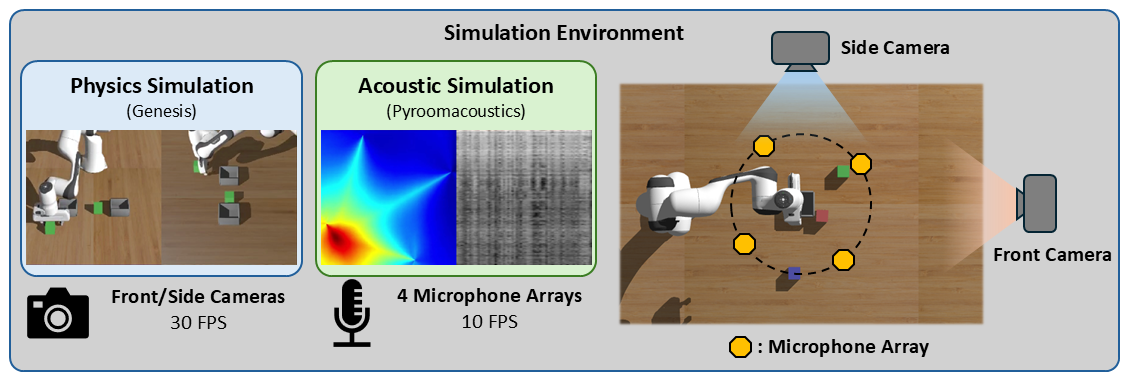
\includegraphics[keepaspectratio, width=14cm]{fig/fig2.png}
		\caption{Simulation settings. 物理シミュレータGenesisと音響シミュレータPyroomacousticsを統合したシミュレーション環境構成．カメラから取得されるRGB画像は30FPSで，Microphone Arrayから取得される音情報は10FPSで更新される．Franka Emika Pandaの500mm正面を作業空間の中心とし，その中心から半径300mmの円周上に4つのマイクロフォンアレイを等間隔に配置した．Side CameraとFront Cameraの2台のカメラは作業空間の中心を映すように設置した．}
		\label{fig:fig2}
	\end{figure}


\subsection{シミュレーション実験結果}
\label{sec:sim_results}
	全タスク・全Policy・全条件の成功率をTable~\ref{tab:results}に，学習ステップ数に対する成功率の推移をFig.~\ref{fig:fig3}に示す．
	以降では，各タスクで明らかになった主要な知見と，4タスクを横断する観察を順に述べる．

	\begin{figure}[t]
		\centering
		\includegraphics[keepaspectratio, width=14cm]{fig/fig3.png}
		\caption{学習ステップ数に対するタスク成功率の変化．4タスクにおける4 Policy（ACT，Diffusion Policy，VQ-BeT，$\pi_0$）のS2A2条件における学習推移を示す．Localization TaskおよびIdentification Taskは10,000 Step毎に最大100,000 Stepまで，Localization \& Identification TaskおよびExploratory Taskは20,000 Step毎に最大200,000 Stepまで評価した．}
		\label{fig:fig3}
	\end{figure}

	\begin{table*}[t]
		\centering
		\scriptsize
		\setlength{\tabcolsep}{4pt}
		\caption{全タスクにおけるタスク成功率（\%）の比較（Mean $\pm$ STD）．各Policy内で最良の値を太字で示す．なお，w/o Spec.はS2A2の入力からSpectrogramを除いたModelであり，w/o Spat.はS2A2の入力からAcoustic Spatial Mapを除いたModelである．また，L \& I TaskはLocalization \& Identification Taskの略称である．}
		\label{tab:results}
		\begin{tabular}{llcccc}
			\hline
			Model & Policy & Localization Task & Identification Task & L \& I Task & Exploratory Task \\
			\hline
			Baseline & ACT & 20.3 $\pm$ 7.2 & 39.3 $\pm$ 4.0 & 11.0 $\pm$ 3.5 & 35.0 $\pm$ 5.3 \\
			 & Diffusion Policy & 13.3 $\pm$ 1.2 & 41.3 $\pm$ 2.5 & 9.3 $\pm$ 6.1 & 26.3 $\pm$ 0.6 \\
			 & VQ-BeT & 12.7 $\pm$ 6.8 & 24.0 $\pm$ 6.9 & 7.7 $\pm$ 1.2 & 17.3 $\pm$ 5.8 \\
			 & $\pi_0$ & 18.3 $\pm$ 2.3 & 32.3 $\pm$ 2.1 & 7.0 $\pm$ 4.0 & 9.0 $\pm$ 1.0 \\
			\hline
			S2A2 & ACT & 73.0 $\pm$ 5.6 & \textbf{76.7 $\pm$ 1.2} & \textbf{78.7 $\pm$ 2.1} & \textbf{77.3 $\pm$ 5.7} \\
			 & Diffusion Policy & 68.0 $\pm$ 3.6 & 67.7 $\pm$ 7.2 & \textbf{89.7 $\pm$ 2.1} & \textbf{44.0 $\pm$ 3.6} \\
			 & VQ-BeT & 40.3 $\pm$ 4.5 & 32.3 $\pm$ 10.0 & \textbf{55.3 $\pm$ 11.7} & \textbf{32.7 $\pm$ 12.7} \\
			 & $\pi_0$ & \textbf{32.0 $\pm$ 9.9} & 73.3 $\pm$ 8.4 & \textbf{45.7 $\pm$ 8.1} & 18.7 $\pm$ 4.2 \\
			\hline
			w/o Spec. & ACT & \textbf{74.7 $\pm$ 4.7} & 44.3 $\pm$ 2.3 & 45.0 $\pm$ 3.6 & 75.3 $\pm$ 5.0 \\
			 & Diffusion Policy & \textbf{68.3 $\pm$ 13.7} & 32.7 $\pm$ 3.1 & 46.0 $\pm$ 5.3 & 37.3 $\pm$ 8.1 \\
			 & VQ-BeT & \textbf{44.7 $\pm$ 5.5} & 32.7 $\pm$ 3.1 & 32.3 $\pm$ 7.5 & 20.0 $\pm$ 20.0 \\
			 & $\pi_0$ & 17.3 $\pm$ 5.0 & 40.0 $\pm$ 11.4 & 14.3 $\pm$ 2.9 & \textbf{26.7 $\pm$ 3.2} \\
			\hline
			w/o Spat. & ACT & 15.3 $\pm$ 4.0 & 74.3 $\pm$ 7.0 & 25.7 $\pm$ 3.1 & 72.3 $\pm$ 8.4 \\
			 & Diffusion Policy & 15.3 $\pm$ 1.2 & \textbf{80.3 $\pm$ 3.8} & 8.7 $\pm$ 3.8 & 6.3 $\pm$ 2.3 \\
			 & VQ-BeT & 12.3 $\pm$ 3.8 & \textbf{49.3 $\pm$ 9.8} & 19.0 $\pm$ 1.0 & 25.0 $\pm$ 3.6 \\
			 & $\pi_0$ & 14.7 $\pm$ 5.7 & \textbf{78.7 $\pm$ 6.0} & 19.7 $\pm$ 3.8 & 9.3 $\pm$ 10.4 \\
			\hline
		\end{tabular}
	\end{table*}


\subsubsection{Localization / Identification Task：単一音響モダリティ依存タスク}
	Localization Taskでは，視覚的に同一の対象を音源位置に基づいて区別する必要がある．アブレーションの結果，Spectrogram Pipelineを除いた条件のモデルはS2A2と同水準の性能を維持した一方で，Acoustic Spatial Map Pipelineを除いた条件のモデルはBaselineと同程度の成功率にとどまった．この対比は，本タスクの判断に寄与する音響情報がAcoustic Spatial Mapに含まれており，Spectrogramからは得られないことを示している．

	Identification Taskでは，運搬対象となる箱を音色の違いに基づいて決定する必要がある．
	Localization Taskとは対照的に，Acoustic Spatial Map Pipelineを除いた条件のモデルがS2A2と同程度の性能を示し，Spectrogram Pipelineを除いた条件のモデルはBaselineを大きく超えなかった．これは，音色識別に必要な情報がSpectrogram側に含まれていることを示している．

	% ただし，VQ-BeTは上記2タスクで他のPolicyと比較して低い成功率にとどまった．VQ-BeTは行動を離散コードに量子化する設計であり，音響情報に応じた搬送先の連続的な位置調整との相性に課題があると考えられる．

	一方で，Localization TaskにおいてAcoustic Spatial Map Pipelineを含まない条件では，複数のPolicyでBaselineと同水準あるいはそれを下回る成功率が観測された．
	この点については~\ref{sec:cross_analysis}節で他タスクの結果と併せて再度議論する．



	% SoundPositionの結果は，Acoustic Spatial Mapが音源定位タスクにおいて十分な情報を提供する音響表現として機能することを示している．
	% ACT と Diffusion Policy はいずれもOurs$_{Spat}$でそれぞれ 74.7\%，68.3\% を達成し，
	% S2A2でも 73.0\%，68.0\% と同等の性能を維持した．
	% 一方，Ours$_{Spec}$は Baseline と同水準にとどまり，
	% 判断に寄与しない音響情報のみを与えても性能向上は得られないことが確認された．
	% Baseline の成功率はいずれの Policy でも 20\% 以下であった．
	% % 解のマルチモーダル性の話
	% 本タスクは二択であり対象選択のみであれば期待値は 50\% であるが，
	% Table~\ref{tab:results} の値は対象選択の正答率ではなく，
	% 把持・搬送・箱投入までを含む全体成功率である．
	% 視覚的に対象を区別できない条件では，誤選択に加えて，
	% 曖昧な入力に対して平均化された行動が生成されて把持段階で失敗するため，
	% 全体成功率はこの水準にとどまる．

	% SoundToneの結果は，Spectrogramが音色識別タスクにおいて十分な情報を提供する音響表現として機能することを示している．
	% ACT と Diffusion Policy ではOurs$_{Spec}$がそれぞれ 74.3\%，80.3\% を達成し，
	% S2A2もこれらと近い水準を示した．
	% 一方，VQ-BeT はOurs$_{Spec}$でも 49.3\% にとどまり，他の Policy と比較して低い水準であった．
	% VQ-BeT は行動を離散コードへ量子化する設計であり，
	% 音色に応じた搬送先の連続的な調整との相性に課題があると考えられる．

	% SoundPosition のOurs$_{Spec}$では，ACT: Ours$_{Spec}$ 15.3\% に対し Baseline 20.3\%というように，Baseline と同水準もしくはそれを下回る Policy が複数見られた．
	% デモンストレーション数が限られた条件下では，判断に寄与しない入力次元を無視する表現の学習が困難となり，結果として最適化を阻害する可能性がある．
	% 不要なモダリティの導入が性能を低下させるという結果は，入力モダリティの選択をタスクの性質に応じて慎重に行うべきことを示しており，~\ref{sec:cross_analysis} で他タスクの結果と併せて再度議論する．

\subsubsection{Localization \& Identification Task：音源位置と音色の統合}
	Localization \& Identification Taskは，音源位置と音色の両方を判断に用いる必要のあるタスクである．
	Baselineの成功率は全Policyで10\%前後にとどまり，視覚情報のみでは操作対象を特定できないことが確認できる．
	アブレーションでは，Acoustic Spatial Map PipelineまたはSpectrogram Pipelineのいずれか一方を欠いた条件では，両者を備えるS2A2と比較して成功率が大きく劣化した．
	これは，本タスクにおいて対象物体の選択および搬送先の決定に，音空間情報と音色情報の双方が必要であり，両Pipelineを併せてS2A2 Modelに組み込むことが重要であることを示している．

	特に注目すべきは，S2A2のDiffusion Policyが全実験中最高の成功率を達成した点である．Diffusion Policyが生成するマルチモーダルな行動分布は，本タスクが扱う，音源位置と音色の組合せに伴う複数の行動候補を扱う上で有効に働いたと考えられる．


	% SoundAll タスクは，音源位置と音色の両方が必要な，本研究で最も総合的なタスクである．Baseline の成功率は全Policyで 7〜11\% と低く，視覚情報のみでは操作対象を特定できないことが確認される．Ours$_{Spat}$は ACT で 45.0\%，Diffusion Policy で 46.0\% まで向上するが，音色に応じた箱選択には不十分である．Ours$_{Spec}$も対象物体の選択に必要な情報が不足するため，性能は限定的である．
	% S2A2は，ACT で 78.7\%，Diffusion Policy で 89.7\%，VQ-BeT で 55.3\%，π0 で 45.7\% を達成し，全Policyで他の条件を上回った．この結果は，位置と音色の両方が判断に必要となるタスクでは，対応する両方の入力表現をPolicyに与えることが必要であることを示している．

	% Diffusion PolicyのS2A2が89.7\%と全実験中最高の成功率を達成したことは注目すべき結果である．Diffusion Policyが生成するマルチモーダルな行動分布は，音源の位置と音色を組み合わせた複合的な判断に伴う複数の行動候補を扱ううえで有効に働いた．

\subsubsection{Exploratory Task：探索的行動と音響フィードバック}
	Exploratory Taskでは，外見が同一の2つの缶を順に把持・振動させ，音が発生した方を選択的に運搬する必要があり，能動的な探索行動と，それによって得られる音響フィードバックの活用が要求される．

	このタスクで特徴的なのは，音響情報の活用効率がPolicy間で大きく異なる点である．
	ACTでは，Acoustic Spatial Map PipelineあるいはSpectrogram Pipelineのいずれか一方を含む条件でもBaselineを大きく上回り，両者を併用したS2A2もそれらと同程度の高い成功率を示した．
	本タスクは把持後に音が観測された物体を選ぶため，音空間情報と周波数情報のいずれの音響表現でも条件分岐に必要な情報が得られていると解釈できる．
	一方で，Diffusion Policy・VQ-BeT・$\pi_0$ではS2A2条件でも性能向上が限定的であった．
	本タスクが要求する，条件分岐を含む比較的長時間のタスクの実施において，Policy自体の行動の表現力やMultimodal Policy内での音響特徴の統合方法の設計差がPolicy間の差を生じさせた要因と考えられる．
	% この点は~\ref{sec:cross_analysis}節および~\ref{sec:tsne}節の潜在空間の可視化でさらに議論する．




	% SoundShake タスクの結果は，音響表現の追加が探索的知覚タスクにおいても有効であること，および Policy のアーキテクチャによって有効性が大きく異なることを示している．

	% ACT は音響表現の追加によって明確な性能向上を示した．
	% Ours$_{Spat}$とOurs$_{Spec}$はそれぞれ75.3\%・72.3\%を達成し，S2A2は77.3\%と同等以上の成功率を示した．
	% 本タスクは振動後に音が観測された物体を選択するという過渡的な音響イベントに基づく手がかりが支配的であり，
	% ACT ではいずれの単一音響モダリティでも Baseline を大きく上回った．
	% Baseline でも35.0\%を示しているのは，視覚的・動力学的な把持動作自体は
	% デモンストレーションから学習可能であり，
	% 音情報がなくても2択のうち偶然正解する事例が残るためである．

	% 他のPolicyでは成功率は低い水準にとどまった．
	% Diffusion Policy のS2A2は44.0\%にとどまり，VQ-BeT・$\pi_0$ も同様に低水準であった．
	% SoundShake タスクが要求する「把持 → 振動 → 音響観測 → 条件分岐」という時間的に長い系列にわたる条件分岐の処理において，
	% 音響特徴の時系列統合方法と行動表現の設計がPolicy 間の差を生じさせた要因と考えられる．


\subsubsection{横断的分析}
\label{sec:cross_analysis}
	Table~\ref{tab:results}に示す4タスクにわたる定量結果に加え，Fig.~\ref{fig:fig4}に示すACTやDiffusion Policyの中間層の潜在特徴量をt-SNE~\citep{vandermaaten2008tsne}により2次元へ射影した結果を併せて参照しつつ，3つの横断的知見を述べる．
	各Policy Networkからの潜在状態の取り出し方および全Policyのt-SNE結果はAppendix~\ref{sec:appendixB}にまとめる．

	\begin{figure}[t]
		\centering
		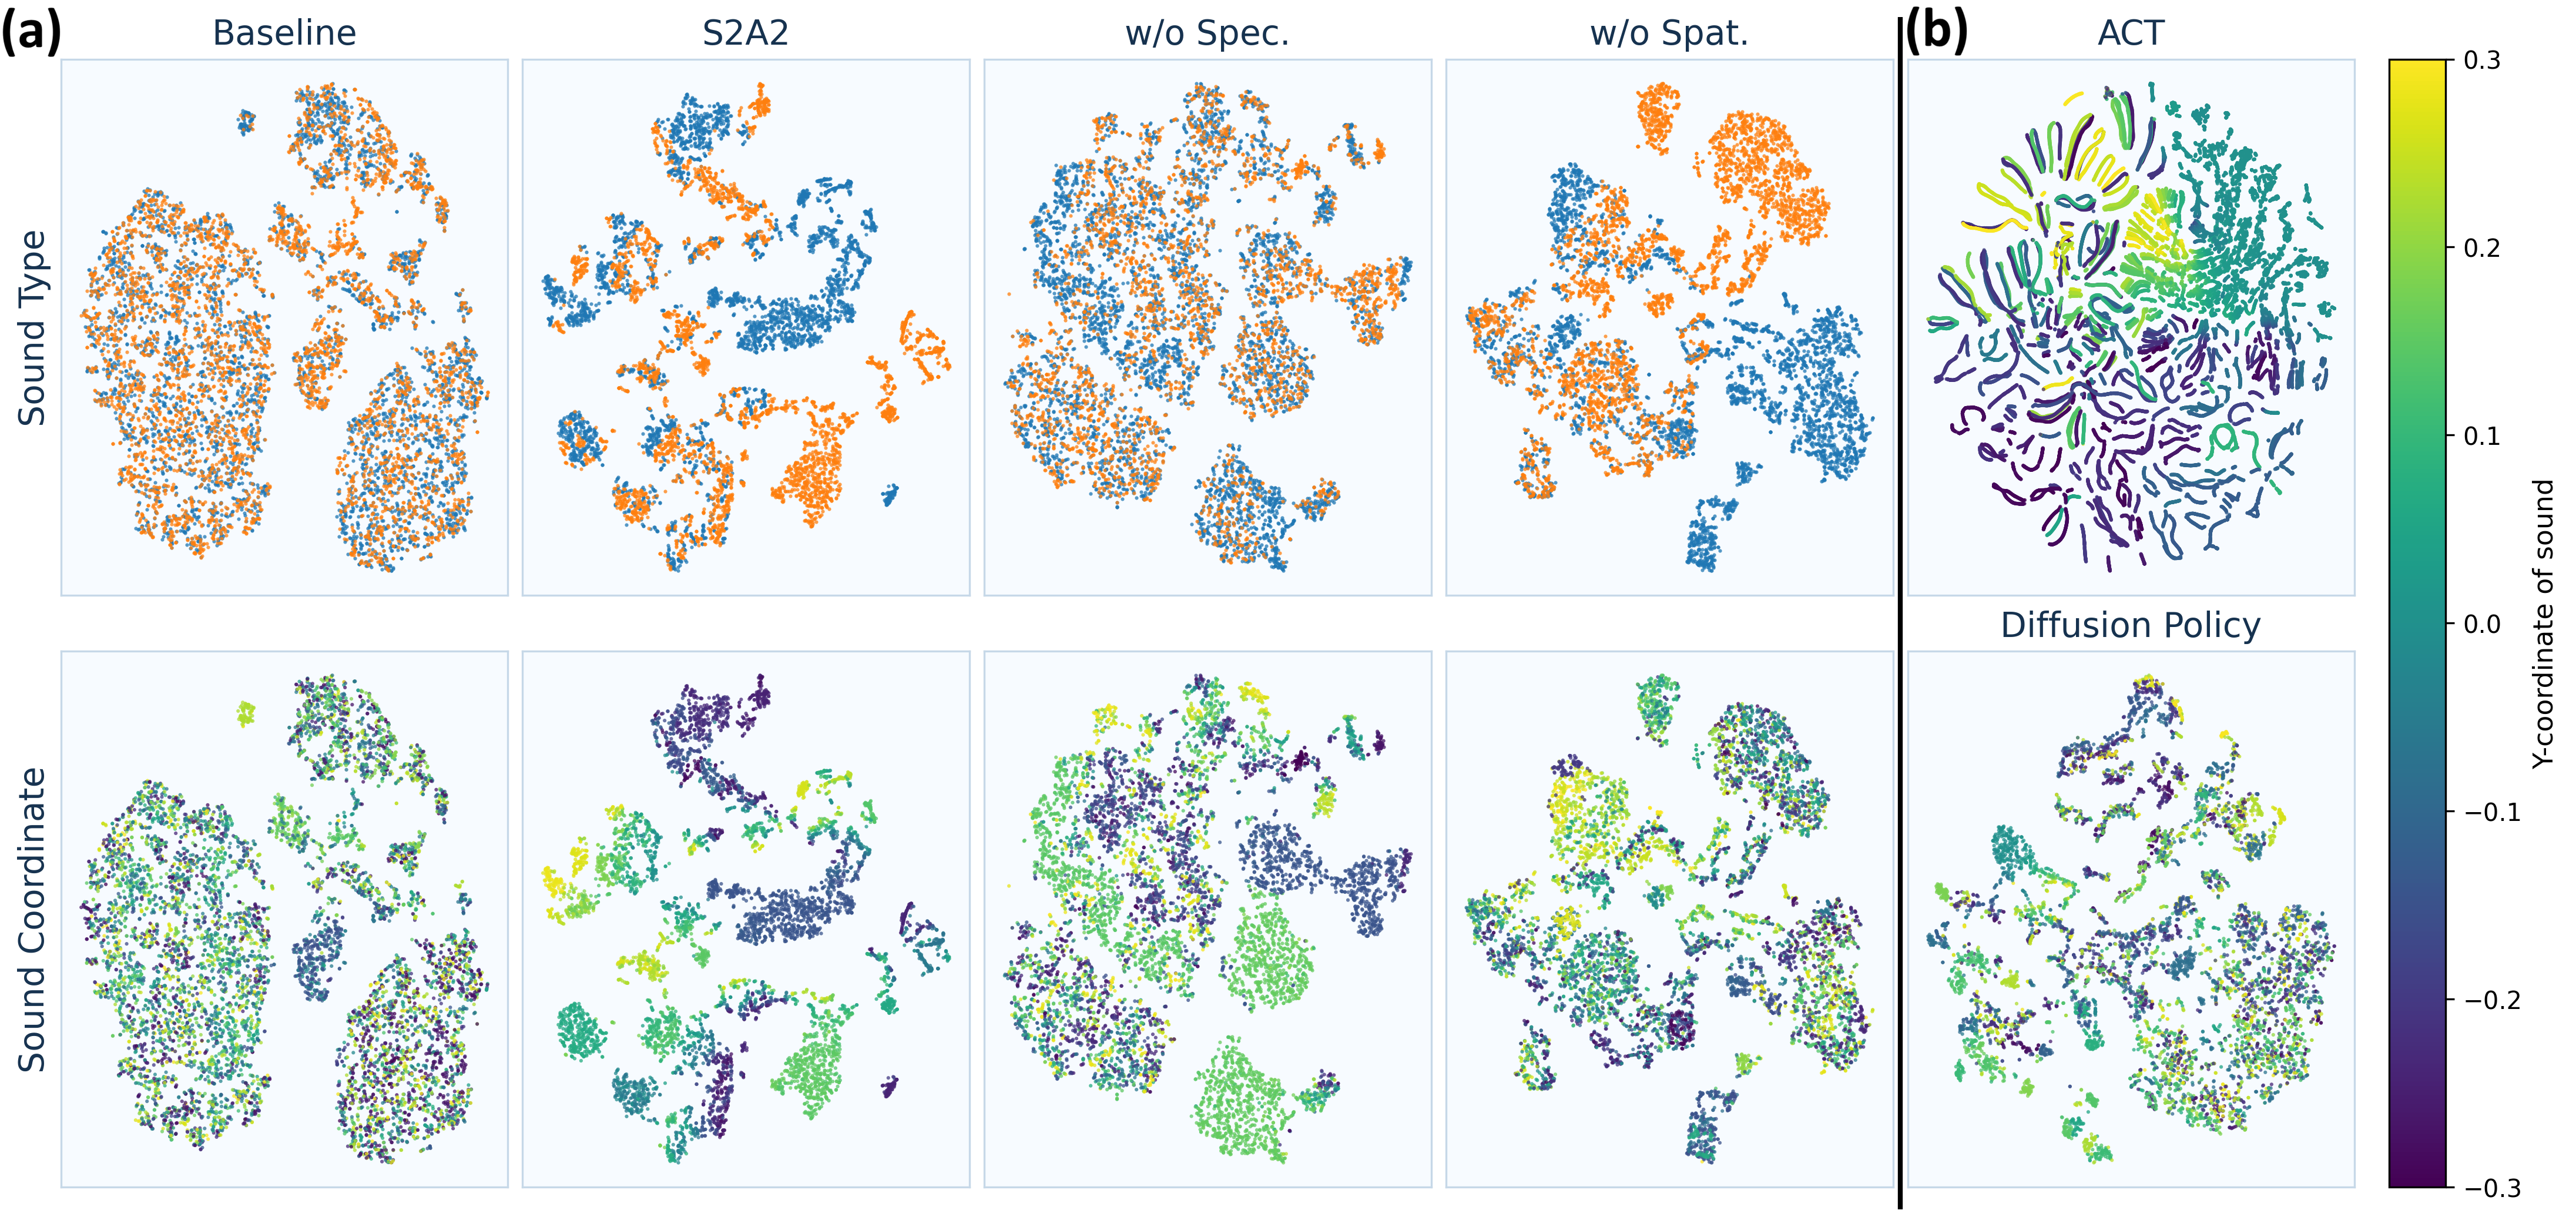
\includegraphics[keepaspectratio, width=14cm]{fig/fig4.png}
		\caption{潜在空間のt-SNE可視化．(a) Diffusion PolicyのLocalization \& Identification Taskにおける，Baseline，S2A2, w/o Spec.，w/o Spat.の比較．t-SNEで分離した潜在特徴量に対して，上段は物体が鳴らしていた音の種類で色分けした図であり，下段は音を鳴らしていた物体のY座標をカラーマップで表現した図．(b) Exploratory TaskにおけるACTとDiffusion Policyの潜在表現t-SNEで分離し，音が鳴る把持対象の物体のY座標をカラーマップで表現した図．全Policyの結果はAppendix~\ref{sec:appendixB}に示す．}
		\label{fig:fig4}
	\end{figure}

	\textbf{音響モダリティとタスク要求の対応．}
	全タスクを通じて，タスクが要求する音響情報に対応したProcessing Pipelineを含む条件で最良の成功率が得られる傾向が一貫して観察された．
	音空間情報のみを要するLocalization Taskや，音色情報のみを要するIdentification Taskでは，それぞれ対応する単一Pipeline条件がS2A2に並ぶ性能を示す一方，両者を要するLocalization \& Identification Taskでは，両Pipelineを備えるS2A2が単独で比較的高いタスク成功率を達成した．
	この対応関係は，Fig.~\ref{fig:fig4}(a)に示す，Diffusion PolicyのLocalization \& Identification Taskにおける潜在空間にも現れている．
	S2A2ではSound TypeとSound Coordinateの双方が比較的よく分離・構造化されているのに対し，Spectrogram Pipelineを除いた条件ではSound Typeがほとんど分離されなくなり，Acoustic Spatial Map Pipelineを除いた条件ではSound Coordinateの構造化が比較的弱くなっていることが確認できる．
	つまり，Acoustic Spatial MapとSpectrogramは潜在空間内で独立した役割を担っていることが定量的，定性的評価の両面から支持される．

	\textbf{不要モダリティの追加による性能低下．}
	タスクに不要なProcessing PipelineをS2A2 Modelに含めた場合，性能がBaselineを下回る事例が複数のPolicy・タスクの組合せで観察された．
	例えばLocalization Taskで判断に寄与しないSpectrogram Pipelineのみを追加した条件や，Exploratory TaskにおけるDiffusion PolicyでSpectrogram Pipelineのみを追加した条件などがその典型例である．
	データ数やデータの多様性が限られたデモンストレーションデータの下では，行動判断に寄与しない入力を無視するようなPolicyを学習することが難しく，結果として冗長な音響情報の入力がPolicyの最適化を阻害した可能性が示唆される．
	したがって，Processing Pipelineの選択はタスクの音響的要請に応じて慎重に行う必要がある．

	\textbf{Policy間の音響情報活用効率の差異．}
	Table~\ref{tab:results}の結果から，音響情報の追加による改善幅はPolicy Networkのアーキテクチャに強く依存することが分かる．
	ACTとDiffusion Policyは多くのタスクで顕著な改善を示した一方，VQ-BeTと $\pi_0$ では改善が限定的なタスクが複数存在した．
	VQ-BeTは行動を離散コードに量子化する設計であり，行動の表現力に制約がある可能性がある．
	また，$\pi_0$は大規模に事前学習されたVision-Language-Action (VLA) Modelであるため，事前学習分布を歪めるような音響特徴の統合方法が性能低下を招いた可能性がある．
	特にFig.~\ref{fig:fig4}(b)に示す，Exploratory Taskにおける潜在空間の可視化では，ACTの潜在空間が音源位置に応じた明瞭な構造を形成するのに対し，Diffusion Policyでは潜在空間の構造化が不明瞭である．
	このような潜在空間の構造化の度合いの差が，結果としてExploratory Taskでの性能差として現れていると解釈できる．
	以上から，音響モダリティの導入方法は，Policy Networkのアーキテクチャに合わせて調整する余地があることが示唆される．




% 	4タスクにわたる結果（Table~\ref{tab:results}）から，以下の3つの横断的知見を抽出する．

% 	\textbf{音響モダリティとタスク要求の対応．}
% 	各タスクにおいて，タスクが要求する音響的能力に対応したモダリティを入力に含む条件が最良の性能を示す傾向が一貫して観察された．
% 	SoundPositionではAcoustic Spatial Mapを含むOurs$_{Spat}$/S2A2が，SoundToneではSpectrogramを含むOurs$_{Spec}$/S2A2が，SoundAll では両者を含むS2A2がそれぞれ最良であった．
% 	この結果は，音響表現の設計がタスク要求と整合する場合にPolicyの判断能力が向上することを示している．

% 	\textbf{不要モダリティの追加による性能低下．}
% 	タスクに不要なモダリティを追加すると，性能が Baseline 以下に低下する場合がある．
% 	SoundPosition におけるOurs$_{Spec}$（ACT: 15.3\%，Baseline: 20.3\%）や，SoundShake における Diffusion Policy のOurs$_{Spec}$（6.3\%，Baseline: 26.3\%）がその典型例である．
% 	限られたデモンストレーションデータのもとでは，判断に不要な入力次元を無視する表現を学習することが困難となり，	結果としてPolicyの最適化を阻害することが示唆される．

% 	\textbf{Policy間の音響情報活用効率の差異．}
% 	音響情報の追加による改善幅はPolicyによって大きく異なる．
% 	ACT と Diffusion Policy は多くのタスクで大きな改善を示した一方，VQ-BeT と $\pi_0$ では改善が限定的なタスクが複数存在した．
% 	VQ-BeT は行動の離散化に伴う表現力の制約が，$\pi_0$ は大規模事前学習モデルへの音響特徴の統合方法が，それぞれ制約要因となった可能性がある．
% 	この知見は，音響モダリティの統合が万能ではなく，Policyのアーキテクチャに応じた設計が必要であることを示している．

% \subsubsection{潜在空間の可視化}
% \label{sec:tsne}
% 	各Policyの内部表現が音響情報をどのように符号化しているかを定性的に分析するため，行動生成直前に得られる潜在特徴量を t-SNE~\citep{vandermaaten2008tsne}により2次元へ射影して可視化した．各モデルからの潜在状態の取り出し方および全Policyの結果はAppendix~\ref{sec:appendixB}に示す．ここでは，本研究の主張に最も関連する2つの観察をFig.~\ref{fig:fig4}にまとめる．

	% \begin{figure}[t]
	% 	\centering
	% 	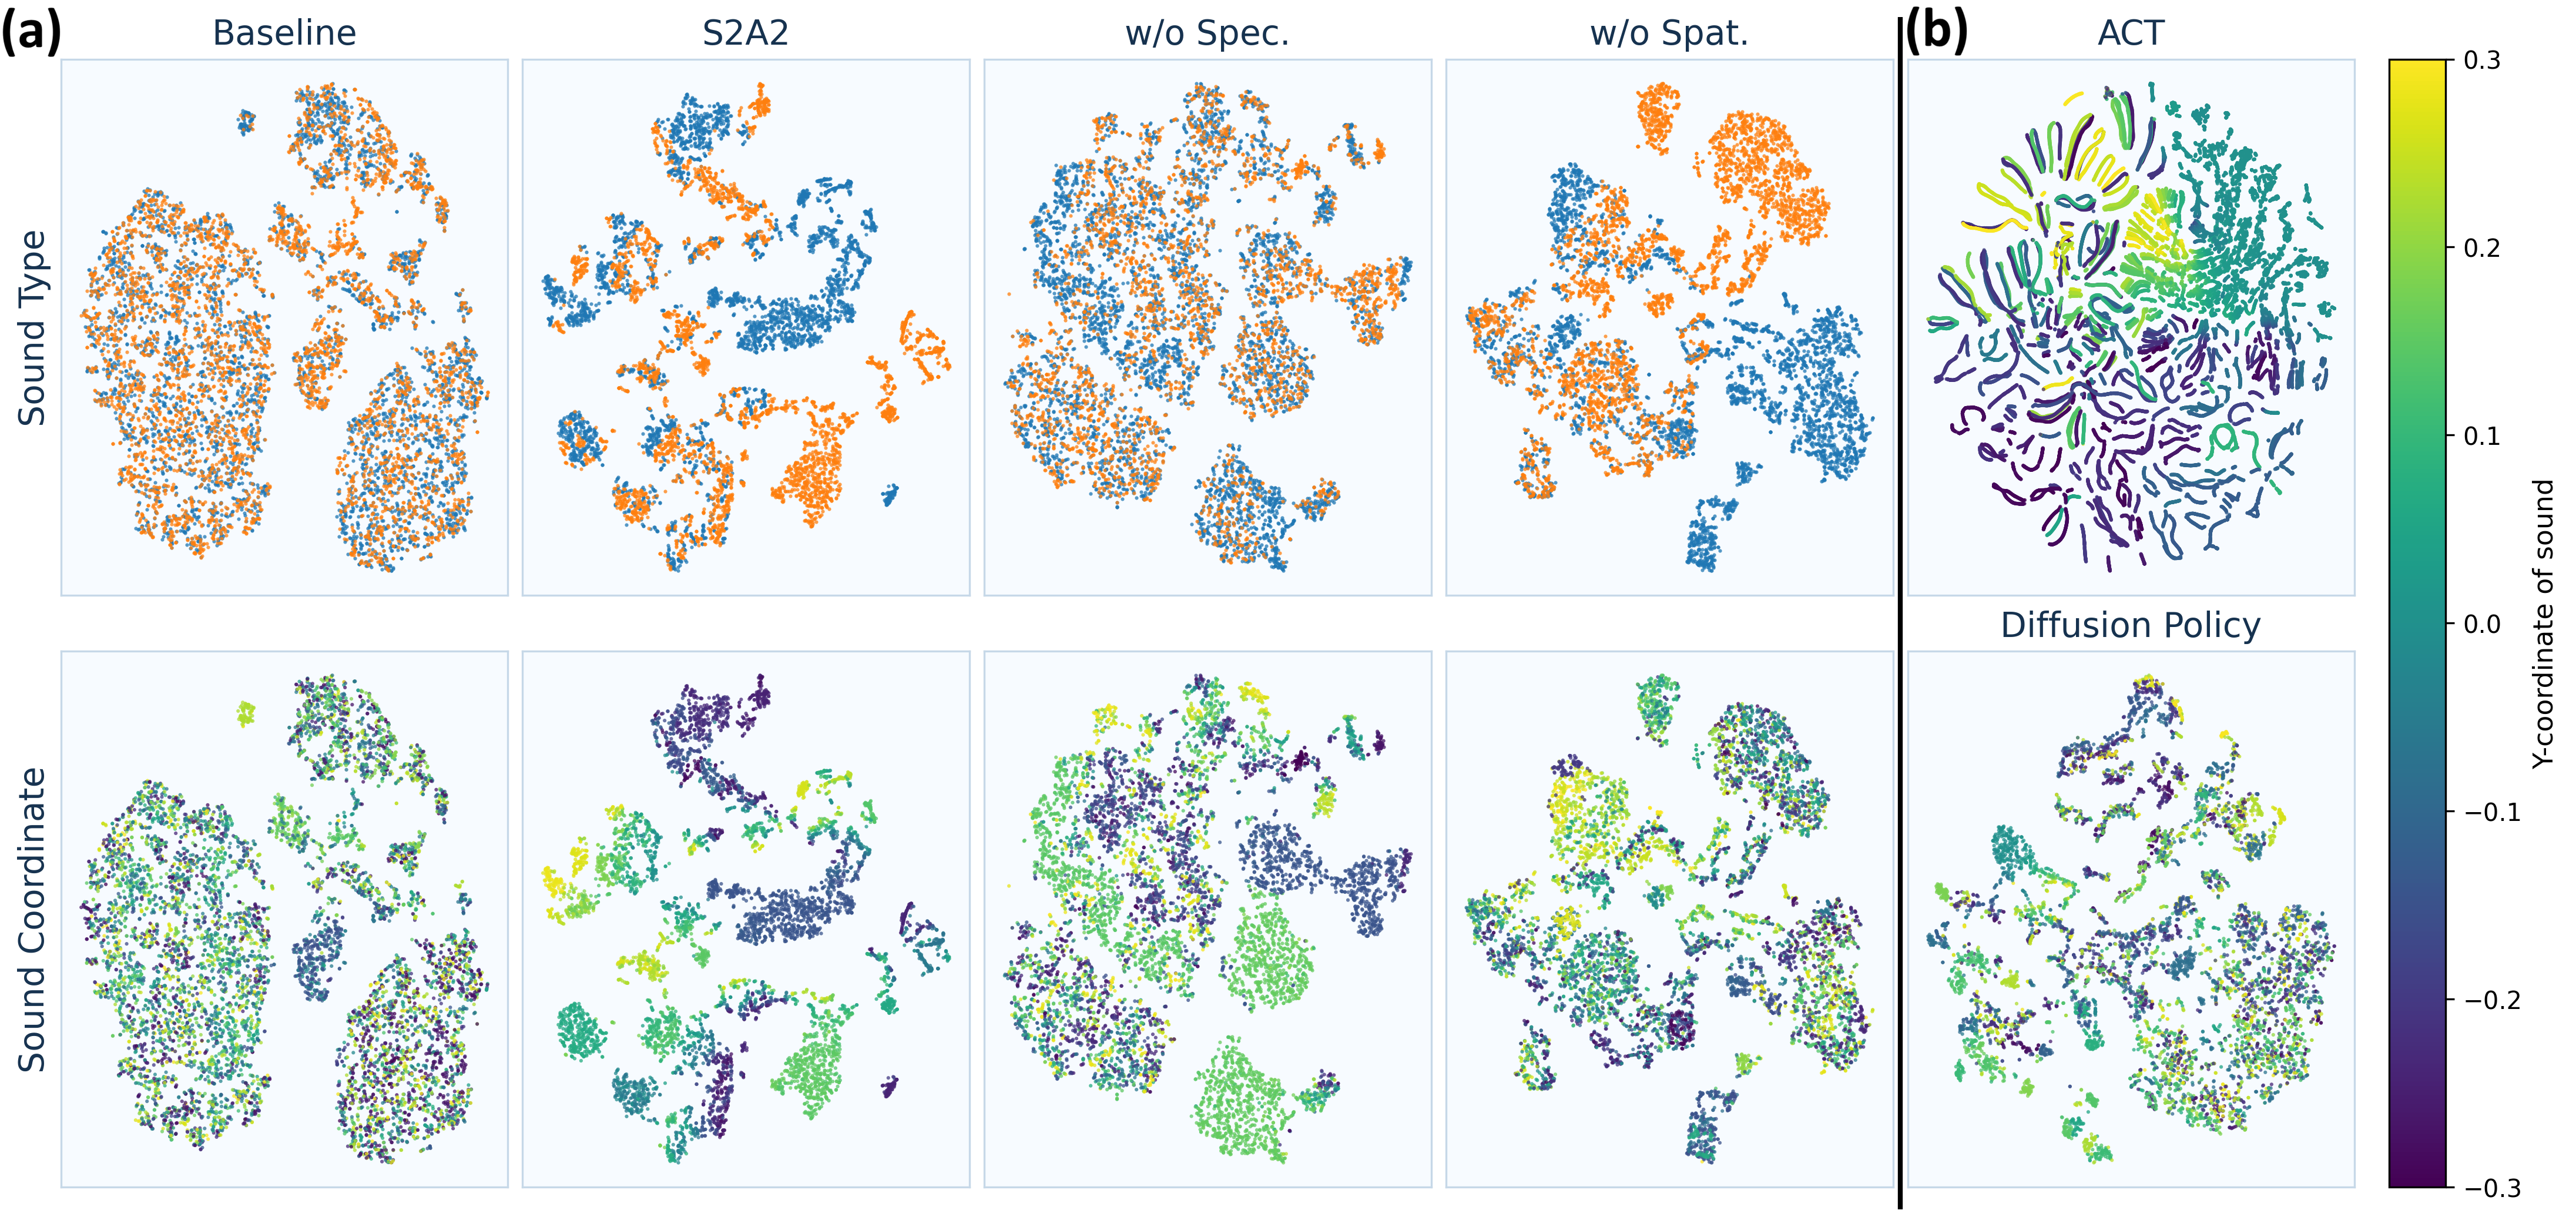
\includegraphics[keepaspectratio, width=14cm]{fig/fig4.png}
	% 	\caption{潜在空間のt-SNE可視化．(a) Diffusion PolicyのSoundAllタスクにおける，Baseline，Ours$_{Spat}$，Ours$_{Spec}$，S2A2の比較．音源位置（Sound Coordinate）および音種（Sound Type）でラベル付けした．S2A2で最も明瞭な構造化が観察される．(b) SoundShakeタスクにおけるACTとDiffusion Policyの音源位置に関する潜在表現の比較．ACTは音源位置に応じた分離が明瞭である一方，Diffusion Policyでは分離が弱い．全Policyの結果はAppendix~\ref{sec:appendixB}に示す．}
	% 	\label{fig:fig4}
	% \end{figure}

% 	\textbf{(a) S2A2における潜在空間の構造化（Diffusion Policy，SoundAll）．}
% 	Fig.~\ref{fig:fig4}(a)はDiffusion PolicyのSoundAllタスクにおける各条件の潜在空間を示す．Baselineではいずれのラベル（音源位置・音種）でも一貫した分離が見られない．Ours$_{Spat}$ではAcoustic Spatial Mapが入力されるため，音源位置に対応した分離が観察される一方，音種の分離は不明瞭である．逆にOurs$_{Spec}$ではSpectrogramにより音種の分離が現れるが，音源位置の分離は限定的である．S2A2ではAcoustic Spatial MapとSpectrogramを併用した結果，音源位置と音種の双方に対応した構造化が確認できる．この観察は，SoundAllタスクにおいてS2A2が89.7\%という最高成功率を達成したという定量的結果（Table~\ref{tab:results}）と整合する．

% 	\textbf{(b) Policy間の差：SoundShakeにおける空間情報の保持．}
% 	Fig.~\ref{fig:fig4}(b)はSoundShakeタスクにおけるACTとDiffusion Policyの潜在空間を音源位置でラベル付けして示したものである．ACTでは音源位置に応じた明瞭な分離が見られる一方，Diffusion Policyでは分離が著しく弱い．SoundShakeタスクではACTのS2A2が77.3\%，Diffusion PolicyのS2A2が44.0\%とPolicy間で大きな性能差が生じているが，この差は，ACTが音源の空間情報を潜在表現として保持できているのに対し，Diffusion Policyでは音響的手がかりが潜在空間に十分に符号化されていないことに対応していると解釈できる．

% 	これらの観察は，Table~\ref{tab:results}の定量的結果と整合しており，各音響モダリティが担う役割の違い，およびPolicyごとの音響情報活用能力の違いを定性的に支持している．






\subsection{実機実験}
\label{sec:real}
	シミュレーションで得られた知見が実環境においても再現されるかを検証するため，実機実験を実施した．
	ロボットにはALOHA~\citep{act}タイプの双腕マニピュレータオープンソースロボットILOHAの右腕のみを用いた．
	マニピュレータを構成する6関節と1自由度のグリッパーを状態・行動として扱ったため，状態・行動はいずれも7次元である．
	視覚情報は俯瞰視点およびマニピュレータのエンドエフェクタに装着したRealSenseカメラから取得した画像をクロップ・リサイズして $224\times224$ のRGB画像として用いた．
	音響情報の取得には円形マイクロフォンアレイTAMAGO-03を4台用いた．
	各アレイは半径35mmの円周上に8素子のマイクロフォンを備える．
	アレイは作業空間を取り囲むように，俯瞰視点で短辺0.6m，長辺1.2mの長方形の各頂点に配置した．
	サンプリング周波数は16kHzとした．

	評価対象タスクには，Localization Taskが要求する能力と，Identification Taskが要求する能力の双方を要求するLocalization \& Identification Taskに加えて，能動的探索を要するExploratory Taskの2種類を選択した．
	Localization \& Identification Taskでは，音源としてBuffalo製の小型スピーカを2つ用いた．
	マニピュレータが把持しやすいよう，スピーカ側面に黄緑色の養生テープを巻き付け，半径約40mm，幅25mmの持ち手を形成した．
	スピーカの搬送先の2つの箱は，黒色で外寸 $60\times90\times90$\,mm であり，それぞれテーブルの両端から280mmの位置に固定した．
	
	Exploratory Taskでは，外観が同一の黒い空き缶を2つ用意した．
	各缶は高さ135mm，直径は上部40mmから下部66mmである．2つの缶のうち一方にのみ金属製ナット3個を封入し，把持して振った際に音が発生するようにした．
	搬送先の灰色の箱は $95\times145mm\times230$\,mmであり，机の中央，ロボット正面に設置した．
	評価Policyには，シミュレーションで両タスクとも安定した性能を示したACTを採用し，S2A2とBaselineを比較した．
	各条件についてデモンストレーションデータを100エピソード収集し，10万ステップの学習を行ったうえで，100回の試行により成功率を評価した．

	各条件のタスク成功率をFig.~\ref{fig:fig5}(b)に示す．
	Localization \& Identification TaskにおいてACTのS2A2は72\%の成功率を示した一方，Baselineは5\%にとどまった．
	Exploratory TaskにおいてもS2A2は50\%の成功率を達成し，Baselineの12\%を上回った．
	いずれのタスクでも，視覚情報のみでは解けない条件に対してS2A2が有効であるというシミュレーションでの知見が，実環境においても再現された．

	実環境には，複雑な音の反射，背景雑音，ロボット駆動系から生じる機械的振動など，シミュレーションでは完全には再現できない音響的外乱が存在する．
	それにもかかわらずS2A2が実機上で機能した要因として，Acoustic Spatial Mapが外乱の影響に比較的ロバストな方向尤度の分布として空間情報を保持していること，およびSpotforming/NMFによる前処理が複数アレイ間で共通して観測される成分のみを残すことで，雑音と局所的なサイドローブを抑制していることが挙げられる．

	\begin{figure}[t]
		\centering
		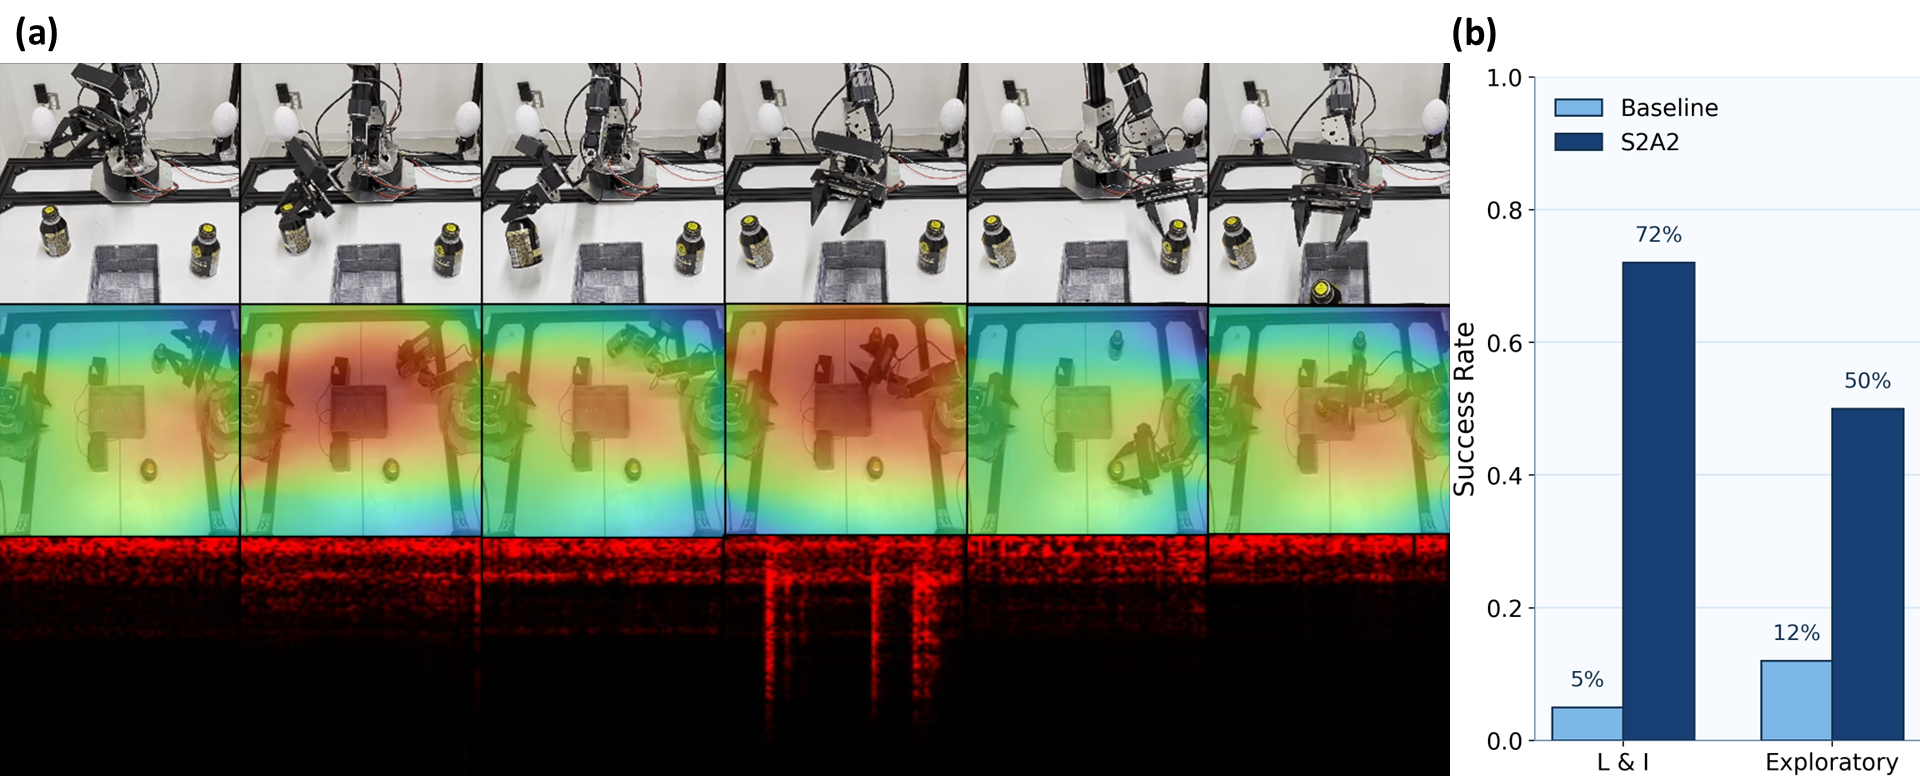
\includegraphics[keepaspectratio, width=14cm]{fig/fig5.png}
		\caption{実機実験の実行例．(a) 上段はExploratory Task実行時のロボットの様子．中段はAcoustic Spatial Mapをチャンネル方向に加算してカラーマップとして表示し，俯瞰視点のカメラ画像に重ね合わせた画像．下段はSpectrogramをRGB画像のRチャンネルに入力し可視化した画像．(b) 実機実験におけるBaselineとS2A2のLocalization \& Identification Task・Exploratory Taskの100試行におけるタスク成功率．}
		\label{fig:fig5}
	\end{figure}

	% 一方で，実機実験においては6軸マニピュレータの関節角度と1自由度のグリッパー開度からなる合計7次元ベクトルをProprioceptionとし，また行動 $a_t$ は6関節位置目標とグリッパー位置目標からなる7次元の位置制御指令である．

% 	シミュレーションで得られた知見が実環境においても再現されるかを検証するため，実機実験を実施した．
% 	ロボットには ALOHA~\citep{act} タイプの双腕型オープンソースロボットILOHAの右腕のみを用いた．
% 	マニピュレータを構成する6関節と1自由度のグリッパーを状態・行動として扱ったため，状態・行動次元はいずれも7である．
% 	視覚情報は俯瞰視点およびILOHAのエンドエフェクタに装着したRealSense カメラから取得した画像を
% 	クロップ・リサイズして $224\times224$ の RGB 画像として用いた．

% 	音響情報の取得には円形マイクロフォンアレイ TAMAGO-03 を4台用いた．
% 	各アレイは半径3.5cmの円周上に8素子のマイクロフォンを備える．
% 	アレイは作業空間を取り囲むように，俯瞰視点で短辺60cm，長辺120cmの長方形の各頂点に配置した．サンプリング周波数は16kHzである．

% 	SoundAll タスクでは，音源としてBuffalo 製の小型スピーカを用いた．
% 	マニピュレータが把持しやすいよう，スピーカ側面に黄緑色の養生テープを巻き付け，
% 	半径40mm，幅25mmの持ち手を形成した．スピーカの搬送先の箱は黒色で外寸$90\times90\times60$\,mm であり，テーブルの端から280mmの位置に設置した．

% 	SoundShake タスクでは，外観が同一の黒い空き缶を2つ用意した．
% 	各缶は高さ135mm，直径は上部40mmから下部66mmである．
% 	2つの缶のうち一方にのみ金属製ナット3個を封入し，把持して振った際にのみ音が発生するようにした．
% 	搬送先の灰色の箱は高さ95mm，短辺145mm，長辺230mmであり，机の中央，ロボット正面に設置した．

% 	評価対象タスクには，シミュレーションにおいて Baseline とS2A2の
% 	差が最も顕著であった SoundAll と，能動的探索を要する SoundShake の2種類を選択した．
% 	評価 Policy には，シミュレーションで両タスクとも安定した性能を示した ACT を採用し，
% 	S2A2と Baseline を比較した．各条件についてデモンストレーションデータを100エピソード収集し，
% 	10万ステップの学習を行ったうえで，100回の試行により成功率を評価した．





% \subsection{実機実験結果}
% 	各条件のタスク成功率をFig.~\ref{fig:fig5}(b)に示す．SoundAll タスクにおいて，ACT のS2A2は 72/100 の成功率を示した一方，Baseline は 5/100 にとどまった．SoundShake タスクにおいても，S2A2は 50/100 を達成し，Baseline の 12/100 を上回った．これらの結果は，視覚情報のみでは解けないタスクに対して，提案手法がシミュレーションで観察された性能向上を実環境でも再現することを示している．
% 	実環境では，反射音，背景雑音，ロボット駆動系から生じる機械的振動など，シミュレーションでは完全に再現できない音響的外乱が存在する．それにもかかわらず，提案手法が実機上で機能した要因として，Acoustic Spatial Mapが単一の推定座標ではなく方向尤度の分布として空間情報を保持していること，および Spotforming/NMF による前処理が複数アレイ間で共通して観測される成分のみを残すことで雑音と局所的なサイドローブを抑制していることが挙げられる．

% 	\begin{figure}[t]
% 		\centering
% 		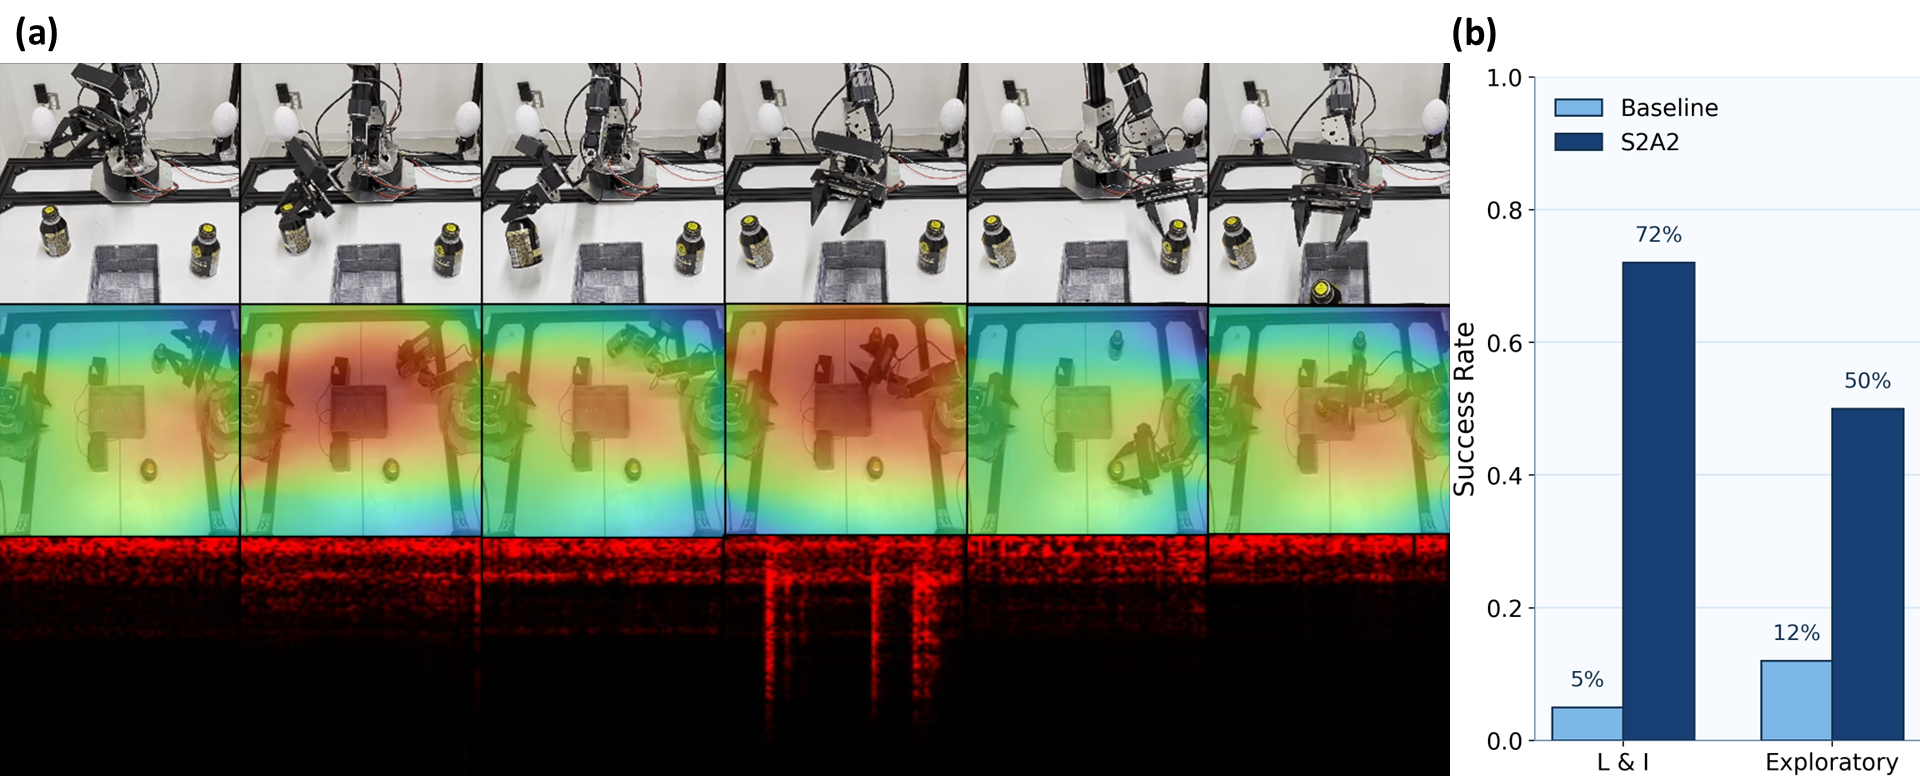
\includegraphics[keepaspectratio, width=14cm]{fig/fig5.png}
% 		\caption{実機実験の実行例．(a) 上段はSoundShakeタスク実行時のロボットの様子．中段は音情報マップをチャンネル方向に加算し，カラーマップとして表示し，それを俯瞰視点のカメラ画像に重ね合わせた画像．下段はSpectrogramをRGB画像のRチャンネルに入力し，可視化した画像．(b) 実機実験におけるBaselineとS2A2のSoundAll・SoundShakeタスクの100試行におけるタスク成功率．}
% 		\label{fig:fig5}
% 	\end{figure}

%===============================================================================








\section{Conclusion}
\label{sec:conclusion}
	本研究では，音源の空間情報を表すAcoustic Spatial Mapと周波数情報を表すSpectrogramを視覚情報と統合したマルチモーダル模倣学習フレームワーク S2A2 を提案した．
	ロボット聴覚分野で発展してきた MUSIC 法による DOA 推定とSpotforming/NMF を模倣学習の入力表現として再定式化し，音源の空間情報と周波数情報を明示的に分離してポリシーに入力するフレームワークを構築した．

	Acoustic-Aware Manipulation Tasks の4タスクと4種の代表的ポリシーにわたる体系的評価から，3つの主要な知見が得られた．
	(1)~タスクが要求する音響的能力に対応したモダリティの入力が性能向上に直結すること，
	(2)~タスクに不要なモダリティの追加が性能を低下させ得ること，
	(3)~音響情報の活用効率はポリシーのアーキテクチャに依存し，
	特に大規模事前学習モデルでは統合方法の設計が重要であることが示された．
	実機実験では，これらの知見が実環境においても再現されることを確認した．

	これらの結果は，音響モダリティが受動的な補助情報ではなく，視覚情報が本質的に曖昧な状況でのロボット操作を可能にする基盤となり得ることを示している．
	提案した Acoustic-Aware Manipulation Tasks と音響表現の設計指針は，音を活用したロボット操作研究の体系的な評価基盤として今後の研究に貢献するものである．

%===============================================================================






\section{Limitations}
	本研究にはいくつかの制限があり，今後の課題として認識している．
	本研究の実機検証は ACT および SoundAll，SoundShake タスクに限定しており，Diffusion Policy，VQ-BeT，$\pi_0$における実環境性能は未検証である．また，シミュレーションと実機との音響特性のギャップを定量化するには至っていない．より広範なPolicy・タスクにわたる実機評価と，sim-to-real ギャップの体系的分析は今後の重要な課題である．

	本研究で扱うタスクでは基本的に目的音源が1〜2種類であったが，多数の異なる音源が同時に存在する複雑な工場環境などへの対応は未検討である．音源分離技術の高度化や，より多数のマイクロフォンアレイの活用が今後の課題となる．

	SoundShakeタスクに代表される探索的行動を要するタスクでは，ロボットが音響情報を取得する以前の初期段階において，把持対象を一意に決定できないマルチモーダルな解の問題が生じる．この問題はACTのTemporal Ensemblingによって顕在化しやすく，能動的な探索戦略や行動サンプリングの改善が必要である．

	実験結果から，音響情報の活用効率はPolicyによって大きく異なることが示された．特に$\pi_0$とVQ-BeTでは改善幅が限定的な条件が見られた．$\pi_0$のような大規模事前学習モデルへの音響情報の効果的な統合方法は，今後の重要な研究課題である．具体的には，音響トークンの挿入位置，バックボーンの凍結範囲，LoRA等の軽量適応，プロンプト設計を検討する必要がある．

	本研究ではPyroomacousticsによる音響シミュレーションを用いたが，複雑な残響，非線形な反射，動的な環境変化など，実環境の音響特性との差異は依然として存在する．より高忠実度の音響シミュレータの活用や，sim-to-real手法~ \citep{multigen2025}の導入が求められる．

	本研究では各タスクに対して100〜200エピソードのデモンストレーションデータを収集したが，実用的な展開においてはより少ないデモンストレーションで学習できることが望ましい．音響情報が学習効率に与える影響の詳細な分析，および少数ショット学習への対応は今後の課題である．

%===============================================================================
% Citations can be made using either \textbackslash citep\{\} or \textbackslash citet\{\}, depending from the appropriateness. To avoid the citation moving to the next line, it is often a good practice to replace the space before with a tilde (\~{}) character.
% Example 1: ``CoRL is the best conference ever~\citep{Gauss1857}.''
% Example 2: ``\citet{Lagrange1788} proved, both theoretically and numerically, that CoRL is the best conference ever.''
\clearpage
% The acknowledgments are automatically included only in the final and preprint versions of the paper.
\acknowledgments{If a paper is accepted, the final camera-ready version will (and probably should) include acknowledgments. All acknowledgments go at the end of the paper, including thanks to reviewers who gave useful comments, to colleagues who contributed to the ideas, and to funding agencies and corporate sponsors that provided financial support.}

%===============================================================================
% no \bibliographystyle is required, since the corl style is automatically used.
\bibliography{main}  % .bib

\clearpage

\appendix
%===============================================================================









\section{Implementation Details}
\label{sec:appendixA}
本章では，S2A2 Modelの実装詳細，音響処理パラメータ，シミュレーション実験と実機実験の差分を示す．

\subsection{Policy Architecture and Hyperparameters}
\label{sec:appendix_architecture}
Table~\ref{tab:policy_architecture}に，各Policy Networkの入力統合方法，エンコーダ，行動生成部，損失関数の概要を示す．表中の\textbf{S2A2}はRGB画像，Acoustic Spatial Map，Spectrogram，Proprioceptionをすべて用いる標準モデルを表す．\textbf{w/o Spat.}はAcoustic Spatial Map Pipelineを除いたモデル，\textbf{w/o Spec.}はSpectrogram Pipelineを除いたモデルである．

\begin{table*}[t]
\centering
\scriptsize
\setlength{\tabcolsep}{3pt}
\caption{S2A2 ModelにおけるPolicy Network別のアーキテクチャ概要．}
\label{tab:policy_architecture}
\begin{tabular}{p{0.13\textwidth} p{0.23\textwidth} p{0.23\textwidth} p{0.21\textwidth} p{0.13\textwidth}}
\hline
Policy & 入力統合 & RGB Encoder & Audio Encoder & 行動生成・損失 \\
\hline
ACT & 各モダリティ特徴マップをトークン化し，Transformer encoderへ入力． & ImageNet事前学習済みResNet-18，$1\times1$畳み込みで512次元へ射影． & Spatial/Spectral Encoderはいずれも専用ResNet-18．特徴マップを512次元トークンへ射影． & Transformer decoderが行動チャンクを出力．L1損失 + KL損失． \\
Diffusion Policy & 各特徴量とProprioceptionをconcatし，U-Netのグローバル条件に使用． & ResNet-18 + Spatial Softmax．カメラごとに独立． & 専用ResNet-18 + Spatial Softmax． & Conditional U-Netがノイズを予測．DDPMノイズ予測MSE． \\
VQ-BeT & 各特徴量，Proprioception，action query tokenをGPT-style networkへ入力． & ResNet-18 + Spatial Softmax． & 専用ResNet-18 + Spatial Softmax． & 離散コード分類 + 連続オフセット予測．Focal Loss + L1損失． \\
$\pi_0$ & RGB，音響，言語トークンをprefixへ，状態・行動・時刻をsuffixへ入力． & PaliGemma画像エンコーダ． & 専用ResNet-18後，$1\times1$畳み込みでPaliGemma次元へ射影． & Gemma expertがflow matchingで行動列を生成．速度場MSE． \\
\hline
\end{tabular}
\end{table*}

Table~\ref{tab:hyperparams}に，各Policyの主要な学習ハイパーパラメータを示す．ネットワーク構造に強く依存する項目は，Policyごとに分けて記載した．

\begin{table*}[t]
\centering
\scriptsize
\setlength{\tabcolsep}{3pt}
\caption{各Policy Networkの学習ハイパーパラメータ．}
\label{tab:hyperparams}
\begin{tabular}{p{0.18\textwidth} p{0.18\textwidth} p{0.20\textwidth} p{0.20\textwidth} p{0.17\textwidth}}
\hline
項目 & ACT & Diffusion Policy & VQ-BeT & $\pi_0$ \\
\hline
Optimizer & AdamW & Adam & Adam & AdamW \\
Learning rate & $1.0\times10^{-5}$ & $1.0\times10^{-4}$ & $1.0\times10^{-4}$（VQ-VAE: $1.0\times10^{-3}$） & $2.5\times10^{-5}$ \\
Weight decay & $1.0\times10^{-4}$ & $1.0\times10^{-6}$ & $1.0\times10^{-6}$（VQ-VAE: $1.0\times10^{-4}$） & $1.0\times10^{-2}$ \\
Scheduler & なし & cosine，warmup 500 steps & warmup 500 steps，VQ-VAE 20,000 steps & cosine decay，warmup 1,000 steps，decay 30,000 steps，final LR $2.5\times10^{-6}$ \\
Batch size & 8 & 32 & 32 & 4 \\
Observation history & 1 & 2 & 5 & 1 \\
Action horizon & $H_{\mathrm{act}}=100$ & $H_d=16$，実行8 steps & $H_q=5$，query token数3 & $H_\pi=50$ \\
Model size & Transformer dim 512，8 heads，encoder 4層，decoder 1層 & U-Net channels $(512,1024,2048)$，DDPM steps 100 & GPT dim 512，8層，8 heads，RVQ 2層，codebook size 16 & flow matching inference 10 steps \\
Normalization & 画像・状態・行動: mean/std & 画像: mean/std，状態・行動: min/max & 画像: identity，状態・行動: min/max & 画像: identity，状態・行動: mean/std \\
Precision & FP32 & FP32 & FP32 & BF16 mixed precision \\
\hline
\end{tabular}
\end{table*}




\subsection{Audio Processing Parameters}
\label{sec:appendix_audio_params}
Table~\ref{tab:audio_params}に，シミュレーションで用いた音響処理パラメータを示す．標準条件では，4台のマイクロフォンアレイを用い，音響表現を10 FPSで更新する．Acoustic Spatial MapとSpectrogramはいずれも$224\times224$にリサイズしてPolicyへ入力する．

\begin{table}[t]
\centering
\scriptsize
\caption{シミュレーション音響処理パラメータ．}
\label{tab:audio_params}
\begin{tabular}{ll}
\hline
項目 & 値 \\
\hline
Sampling rate & 16 kHz \\
STFT FFT length / overlap & 512 / 50\% \\
Audio window & 1.0 s \\
Number of arrays $n$ & 4 \\
Microphones per array / radius & 8 / 3.5 cm \\
Array placement radius & 30 cm \\
Room size / reflection order & $10,\mathrm{m}\times10,\mathrm{m}\times3,\mathrm{m}$ / 3 \\
MUSIC source number & 3 \\
Audio update rate & 10 FPS \\
NMF components / threshold & 50 / $1.6\times10^{-3}$ \\
Spectrogram range / normalization & 0--8000 Hz / min--max \\
Distance attenuation & $d_{\mathrm{floor}}=10.0,\mathrm{m}$，$\gamma=1.0$ \\
\hline
\end{tabular}
\end{table}



\subsection{Sensitivity Analysis of Audio Representation}
\label{sec:appendix_sensitivity}
Fig.~\ref{fig:appendixA}に，音響表現に関する感度分析結果を示す．評価にはACTのS2A2設定を用いた．

\begin{figure}[t]
\centering
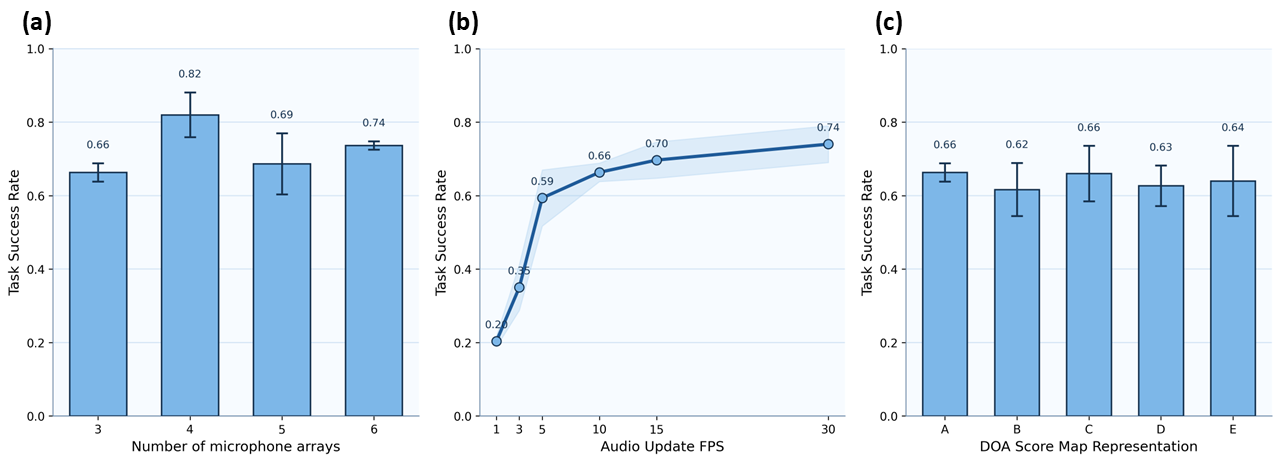
\includegraphics[keepaspectratio, width=14cm]{fig/figb.png}
\caption{音響表現の感度分析．(a) マイクロフォンアレイ数の影響．(b) 音情報の更新FPSの影響．(c) Acoustic Spatial Mapの表現方法の比較．}
\label{fig:appendixA}
\end{figure}

\paragraph{マイクロフォンアレイ数の影響．}
Localization Taskにおいて，マイクロフォンアレイ数$n$を変化させた際の成功率をFig.~\ref{fig:appendixA}(a)に示す．$n=4$のとき成功率が最大となったため，本研究ではこれを標準設定とした．アレイ数が少ない場合はDOA推定に必要な空間的制約が不足し，多すぎる場合は冗長な入力チャンネルが増えることでPolicyの学習が不安定になる傾向が見られた．

\paragraph{音情報の更新FPSの影響．}
Acoustic Spatial MapとSpectrogramの更新頻度を1--30 FPSの範囲で変化させた結果をFig.~\ref{fig:appendixA}(b)に示す．5 FPSを超えると性能が向上し，10 FPS以降でおおむね飽和した．この結果から，本研究では音響情報の標準更新頻度を10 FPSとした．

\paragraph{Acoustic Spatial Map表現の比較．}
Acoustic Spatial Mapの表現方法として，直接投影，特徴量化マップ，時間平滑マップを比較した結果をFig.~\ref{fig:appendixA}(c)に示す．直接投影したAcoustic Spatial Mapが最も高い成功率を示したため，本研究では追加の特徴画像化や時間平滑を行わず，DOAスコアを作業空間へ直接投影した表現を用いた．





\subsection{Differences between Simulation and Real-World Experiments}
\label{sec:appendix_sim_real}
実機実験では，シミュレーションと同じMUSIC，Acoustic Spatial Map生成，Spotforming-NMF，Spectrogram生成の処理系列を用いる．ただし，マイクロフォン配置，ロボット構成，実録音に含まれる雑音に合わせて，Table~\ref{tab:sim_real_diff}に示す差分を導入した．

\begin{table*}[t]
\centering
\scriptsize
\setlength{\tabcolsep}{3pt}
\caption{シミュレーション実験と実機実験の処理差分．}
\label{tab:sim_real_diff}
\begin{tabular}{p{0.23\textwidth} p{0.34\textwidth} p{0.34\textwidth}}
\hline
項目 & シミュレーション & 実機 \\
\hline
Robot state/action & Franka Pandaの9次元状態・9次元位置制御指令 & ILOHA右腕6関節 + グリッパ開度の7次元状態・行動 \\
Camera input & Genesis内の正面・側面RGB画像を$224\times224$で保存 & RealSense画像をクロップ・リサイズして$224\times224$へ変換 \\
Audio input & Pyroomacousticsで音源と部屋反射を生成 & 4台の8chマイクロフォンアレイから16 kHzで実録音 \\
MUSIC source number & 3 & 1 \\
DOA normalization & MUSIC出力を対数化し，方位方向の総和で正規化 & 相対dB化し，60 percentileをノイズ床，15 dBをダイナミックレンジとして正規化 \\
Frequency normalization & なし & 周波数方向に正規化 \\
Acoustic Spatial Map coordinates & シミュレーション作業空間に対応するローカルグリッド & 実機の矩形マイク配置に合わせた$1.4,\mathrm{m}$四方のマップ座標 \\
Distance attenuation & $d_{\mathrm{floor}}=10.0,\mathrm{m}$，$\gamma=1.0$ & $d_{\mathrm{floor}}=0.0,\mathrm{m}$，$\gamma=0.0$ \\
Spectrogram range / normalization & 0--8000 Hz，min--max正規化 & 0--4000 Hz，2/98 percentile正規化 \\
Audio update & 30 FPS環境中で3フレームごとに更新 & 1秒窓の音声バッファを10 FPSで更新 \\
Array channel order & シミュレーションのアレイ生成順 & 左上，右上，右下，左下 \\
Evaluated policies & ACT，Diffusion Policy，VQ-BeT，$\pi_0$ & ACT，Diffusion Policy \\
ACT inference & temporal ensemble係数0.01，1 step実行 & temporal ensembleなし，30 steps実行 \\
\hline
\end{tabular}
\end{table*}











% 	各ポリシーの学習・モデルパラメータを Table~\ref{tab:hyperparams} に示す．
% 	本文では性能に直接影響する学習率，バッチサイズ，学習ステップ数を述べたため，本節では最適化の詳細，行動系列長，モダリティエンコーダの設定をまとめる．

% 	\begin{table*}[t]
% 		\centering
% 		\scriptsize
% 		\caption{各ポリシーの学習ハイパーパラメータ．}
% 		\label{tab:hyperparams}
% 		\begin{tabular}{p{0.19\textwidth} p{0.18\textwidth} p{0.20\textwidth} p{0.20\textwidth} p{0.17\textwidth}}
% 			\hline
% 			& ACT & Diffusion Policy & VQ-BeT & $\pi_0$ \\
% 			\hline
% 			オプティマイザ & AdamW & Adam & Adam & AdamW \\
% 			学習率 & $1.0\times10^{-5}$ & $1.0\times10^{-4}$ & $1.0\times10^{-4}$（VQ-VAE: $1.0\times10^{-3}$） & $2.5\times10^{-5}$ \\
% 			Weight decay & $1.0\times10^{-4}$ & $1.0\times10^{-6}$ & $1.0\times10^{-6}$（VQ-VAE: $1.0\times10^{-4}$） & $1.0\times10^{-2}$ \\
% 			学習率スケジューラ & なし & cosine，warmup 500 steps & VQ-BeT scheduler，warmup 500 steps，VQ-VAE 20,000 steps & cosine decay，warmup 1,000 steps，decay 30,000 steps，final LR $2.5\times10^{-6}$ \\
% 			Batch size & 8 & 32 & 32 & 4 \\
% 			Action chunk size & 100 & 行動系列長16，実行8ステップ & action query tokenあたりaction chunk長5，action query token 3個 & action chunk長50，実行50ステップ \\
% 			観測履歴長 & 1 & 2 & 5 & 1 \\
% 			視覚バックボーン & ResNet-18，ImageNet事前学習 & ResNet-18，事前学習なし，カメラごとに独立 & ResNet-18，事前学習なし & PaliGemma画像エンコーダ \\
% 			Spatial Encoder & ResNet-18，$n$チャンネル入力，事前学習なし & ResNet-18，$n$チャンネル入力，事前学習なし & ResNet-18，$n$チャンネル入力，事前学習なし & ResNet-18，$n$チャンネル入力，$1\times1$ 畳み込みでPaliGemma次元へ射影 \\
% 			Spectral Encoder & ResNet-18，1チャンネル入力，事前学習なし & ResNet-18，1チャンネル入力，事前学習なし & ResNet-18，1チャンネル入力，事前学習なし & ResNet-18，1チャンネル入力，$1\times1$ 畳み込みでPaliGemma次元へ射影 \\
% 			モデル次元 & Transformer次元512，head数8，encoder 4層，decoder 1層 & Spatial Softmax 32 keypoints，U-Netチャンネル(512, 1024, 2048)，DDPM訓練ステップ100 & GPT次元512，8層，head数8，RVQ 2層，codebook size 16 & 状態・行動の最大次元32，flow matching推論10ステップ \\
% 			学習時メモリ設定 & 32-bit浮動小数点 & 32-bit浮動小数点 & 32-bit浮動小数点 & BF16混合精度，gradient checkpointing有効 \\
% 			正規化 & 画像・状態・行動: 平均・標準偏差 & 画像: 平均・標準偏差，状態・行動: 最小最大 & 画像: 恒等変換，状態・行動: 最小最大 & 画像: 恒等変換，状態・行動: 平均・標準偏差 \\
% 			\hline
% 		\end{tabular}
% 	\end{table*}
% 	BF16はbfloat16浮動小数点形式を指す．gradient checkpointingとは，誤差逆伝播時に一部の中間活性を再計算することでGPUメモリ使用量を下げる学習手法である．

% 	シミュレーションで用いた音響処理パラメータを Table~\ref{tab:audio_params} に示す．
% 	標準条件では，4アレイ，音情報10FPS，Acoustic Spatial MapとSpectrogramの両方を用いる．Acoustic Spatial Mapに対する追加のガウシアン平滑化，時間平滑化，特徴画像化は行わない．

% 	\begin{table}[t]
% 		\centering
% 		\scriptsize
% 		\caption{シミュレーション音響処理パラメータ．}
% 		\label{tab:audio_params}
% 		\begin{tabular}{lc}
% 			\hline
% 			項目 & 値 \\
% 			\hline
% 			サンプリング周波数 & 16 kHz \\
% 			STFT FFT長 / オーバーラップ & 512 / 50\% \\
% 			音響処理窓 & 1.0 s \\
% 			マイクロフォンアレイ数 $n$ & 4 \\
% 			各アレイのマイク数 / 半径 & 8 / 3.5 cm \\
% 			アレイ配置半径 & 30 cm \\
% 			部屋サイズ / 反射次数 & $10\,\mathrm{m}\times10\,\mathrm{m}\times3\,\mathrm{m}$ / 3 \\
% 			MUSIC推定音源数 & 3 \\
% 			音情報更新頻度 & 10 FPS \\
% 			NMF成分数 / 閾値 & 50 / $1.6\times10^{-3}$ \\
% 			Spectrogram表示帯域 / 正規化 & 0--8000 Hz / min--max \\
% 			距離減衰 $d_{\mathrm{floor}},\gamma$ & 10.0 m，1.0 \\
% 			\hline
% 		\end{tabular}
% 	\end{table}


% 	また，Fig.~\ref{fig:appendixA}に，提案手法におけるハイパーパラメータの感度分析結果を示す．

% 	\begin{figure}[t]
% 		\centering
% 		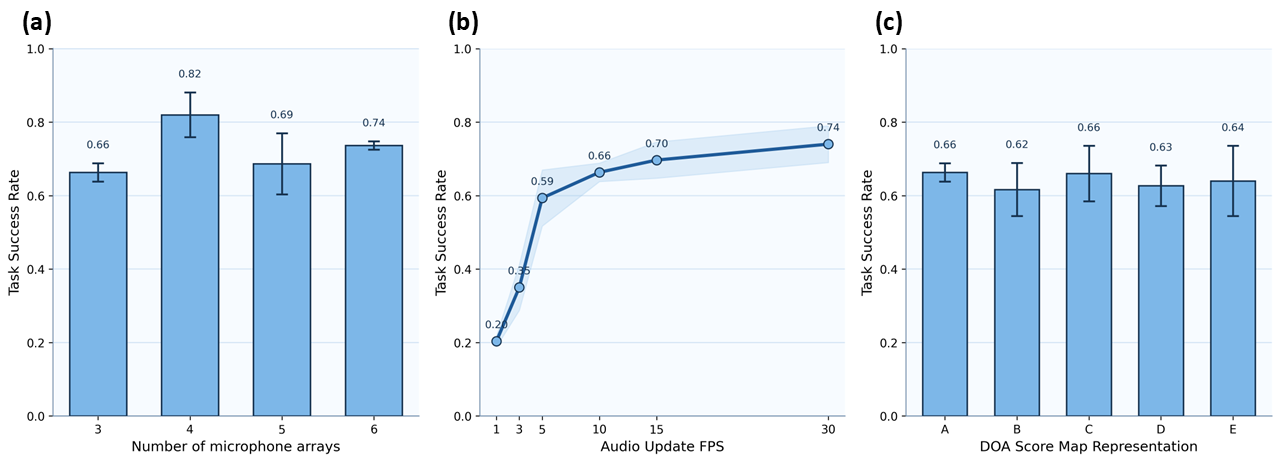
\includegraphics[keepaspectratio, width=14cm]{fig/figb.png}
% 		\caption{ハイパーパラメータの感度分析．(a) マイクロフォンアレイ数の影響．(b) 音情報の更新FPSの影響．(c) Acoustic Spatial Mapの表現方法の比較．}
% 		\label{fig:appendixA}
% 	\end{figure}

% \subsection{マイクロフォンアレイ数の影響}
% \label{sec:appendixA1}
% 	SoundPositionタスクに相当する条件において，マイクロフォンアレイ数 $n$ を変化させた際のタスク成功率の変化をFig.~\ref{fig:appendixA}(a)に示す．評価にはACTのS2A2条件を用いた．$n=4$ のとき成功率が最大値を示したため，本論文の実験ではこれを標準設定とした．アレイ数が少ない場合はDOA推定精度が低下し，多すぎる場合は冗長な情報によるモデルの混乱が生じる傾向が見られた．

% \subsection{音情報の更新FPSの影響}
% \label{sec:appendix_sensitivity}
% 	Acoustic Spatial MapとSpectrogramの更新頻度を1〜30FPSの範囲で変化させた際の成功率変化をFig.~\ref{fig:appendixA}(b)に示す．評価にはACTのS2A2条件とSoundPositionタスクを用いた．5FPSを超えると性能が急激に向上し，10FPS以降で飽和する傾向が確認された．この結果から，動的な把持動作に対して十分な頻度での音響情報更新が重要であることが示された．

% \subsection{音響表現の比較}
% \label{sec:appendixA3}
% 	Acoustic Spatial Mapの表現方法として，直接投影，特徴量化マップ，時間平滑Acoustic Spatial Mapの3種類を比較した結果をFig.~\ref{fig:appendixA}(c)に示す．評価にはACTとSoundPositionタスクを用いた．直接投影したAcoustic Spatial Mapが他の表現を一貫して上回る成功率を達成しており，事前処理を加えることなく生のDOA情報を使用することが有効であることが示された．

% \subsection{シミュレーション実験と実機実験の処理差分}
% \label{sec:appendixA4}
% 	実機実験では，シミュレーションと同じMUSIC，Acoustic Spatial Map生成，Spotforming-NMF，Spectrogram生成の処理系列を用いる．ただし，実環境のマイクロフォン配置，ロボット構成，実録音に含まれる雑音に合わせて，Table~\ref{tab:sim_real_diff} の処理とパラメータを用いる．
% 	実機ではILOHAの単腕構成を用い，右腕6関節とグリッパー開度の合計7次元を状態・行動として扱った．
% 	そのため，シミュレーションのFranka Pandaにおける9次元状態・9次元行動とは次元が異なる．
% 	また，実機評価のACTでは時間アンサンブルを無効化し，1回の推論で得たチャンクのうち30ステップを順に実行した．

% 	\begin{table*}[t]
% 		\centering
% 		\scriptsize
% 		\caption{シミュレーション実験と実機実験の処理差分．}
% 		\label{tab:sim_real_diff}
% 		\begin{tabular}{p{0.20\textwidth} p{0.36\textwidth} p{0.36\textwidth}}
% 			\hline
% 			項目 & シミュレーション & 実機 \\
% 			\hline
% 			ロボット状態・行動 & Franka Pandaの9次元状態・9次元位置制御指令 & ILOHA の右腕6関節 + 右グリッパからなる7次元状態・行動 \\
% 			カメラ & Genesis内の正面・側面RGB画像を $224\times224$ に保存 & RealSense画像をクロップ・リサイズして $224\times224$ に変換 \\
% 			音信号 & Pyroomacousticsで音源と部屋反射を生成 & 4台の8chマイクロフォンアレイから16kHzで実録音 \\
% 			MUSIC推定音源数 & 3 & 1 \\
% 			DOAスペクトル & MUSIC出力を対数化し，方位方向の総和で正規化 & 相対dB化，60パーセンタイルをノイズ床，15dBをダイナミックレンジとして正規化 \\
% 			DOA周波数正規化 & なし & 周波数方向に正規化 \\
% 			Acoustic Spatial Map座標 & シミュレーション作業空間に対応するローカルグリッド & 実機の矩形マイク配置に合わせた $1.4\,\mathrm{m}$ 四方のマップ座標 \\
% 			距離減衰 & $d_{\mathrm{floor}}=10.0\,\mathrm{m}$，$\gamma=1.0$ & $d_{\mathrm{floor}}=0.0\,\mathrm{m}$，$\gamma=0.0$（距離減衰なし） \\
% 			統合マップ平滑化 & ガウシアンフィルタ $\sigma=1.0$ & ガウシアンフィルタ $\sigma=1.0$ \\
% 			Spectrogram帯域・正規化 & 0--8000 Hz，min--max正規化 & 0--4000 Hz，2/98パーセンタイル正規化 \\
% 			音情報更新 & 30FPS環境中で3フレームごとに更新（10FPS） & 1秒窓の音声バッファを10FPSで更新 \\
% 			チャンネル順序 & シミュレーションのアレイ生成順 & 左上，右上，右下，左下の順序 \\
% 			評価対象Policy & ACT，Diffusion Policy，VQ-BeT，$\pi_0$ & ACT，Diffusion Policy \\
% 			実機評価時ACT設定 & シミュレーション評価ではtemporal ensemble係数0.01，実行1 step & temporal ensembleなし，実行30 steps \\
% 			\hline
% 		\end{tabular}
% 	\end{table*}







%===============================================================================
\section{Additional Latent Space Visualizations}
\label{sec:appendixB}

	本節では，~\ref{sec:cross_analysis}で示した本文中のFig.~\ref{fig:fig4}に掲載しきれなかったPolicy・タスクの組み合わせについて追加 t-SNE プロットを示す．

\subsection{潜在状態の抽出方法}
\label{sec:appendixB1}
	各Policyは異なる構造を持つため，潜在状態として用いる特徴量も異なる．本研究では，各Policyにおいて行動生成の直前に得られる中間表現を潜在状態として抽出した．具体的には，ACTではTransformer decoderの出力を，Diffusion PolicyではU-Netの最終畳み込み層の直前に位置するボトルネック層直後の特徴量を，VQ-BeTではGPTスタイルのpolicy networkが出力する特徴量のうちaction queryトークンに対応する位置の表現を，$\pi_0$では最終的な行動射影に入力されるsuffix側の出力をそれぞれ用いた．いずれのPolicyもaction chunkを出力する設計であるため，各エピソードについて行動ステップ方向（チャンク内の時刻方向）に平均をとり，1エピソードあたり1つの潜在ベクトルを得たうえで t-SNE による次元削減を行った．

\subsection{Policy別の追加可視化結果}
\label{sec:appendixB2}
	Fig.~\ref{fig:appendixB_act}〜Fig.~\ref{fig:appendixB_pi0}にACT，Diffusion Policy，VQ-BeT，$\pi_0$それぞれについての全タスクにおける t-SNE プロットを示す．各プロットは，タスク成功・失敗，音源位置，音種をラベルとして色付けしたものである．S2A2条件ではOurs$_{Spat}$・Ours$_{Spec}$・Baselineに比べて，対応するラベルに応じた構造化された分布が観察されやすく，本文の主要な観察と整合している．

	\begin{figure}[t]
		\centering
		\includegraphics[keepaspectratio, width=14cm]{fig/fig_c1.png}
		\caption{ACTにおける t-SNE プロット．全4タスク（SoundPosition，SoundTone，SoundAll，SoundShake）について，成功/失敗，音源位置，音種のラベルで色付けした．}
		\label{fig:appendixB_act}
	\end{figure}
	\begin{figure}[t]
		\centering
		\includegraphics[keepaspectratio, width=14cm]{fig/fig_c2.png}
		\caption{Diffusion Policyにおける t-SNE プロット．}
		\label{fig:appendixB_dp}
	\end{figure}
	\begin{figure}[t]
		\centering
		\includegraphics[keepaspectratio, width=14cm]{fig/fig_c3.png}
		\caption{VQ-BeTにおける t-SNE プロット．}
		\label{fig:appendixB_vqbet}
	\end{figure}
	\begin{figure}[t]
		\centering
		\includegraphics[keepaspectratio, width=14cm]{fig/fig_c4.png}
		\caption{$\pi_0$における t-SNE プロット．}
		\label{fig:appendixB_pi0}
	\end{figure}


\section{追加の実機実験アニメーション}
\label{sec:appendixC}
ここでは，本文中に掲載できなかった実機実験の様子の図をFig.~\ref{fig:real_li_task}，Fig.~\ref{fig:real_ex_task}として掲載する．

	\begin{figure}[t]
		\centering
		\includegraphics[keepaspectratio, width=14cm]{fig/soundRealAll_r0.png}
		\caption{実環境でACTベースのS2S2 Modelが，Localization \& Identification Taskを実行する様子．}
		\label{fig:real_li_task}
	\end{figure}

	\begin{figure}[t]
		\centering
		\includegraphics[keepaspectratio, width=14cm]{fig/soundRealShake_1.png}
		\caption{実環境でACTベースのS2S2 Modelが，Exploratory Taskを実行する様子．}
		\label{fig:real_ex_task}
	\end{figure}
\end{document}